\documentclass[../main.tex]{subfiles}
\usepackage{slashed}
\usepackage[table]{xcolor}
\usepackage{hhline}
\usepackage{lipsum}

\let\Bbbk\relax
\usepackage{amsmath}
\usepackage{amsfonts}
\usepackage{simpler-wick}

\begin{document}
%\setchapterstyle{kao} % decommentare se non si mette l'immagine
\setchapterimage[6.5cm]{images_ch9/SSB3.jpg}
\setchapterpreamble[u]{\margintoc}
\chapter[Rottura Spontanea di Simmetria]{Rottura Spontanea di Simmetria\footnote{Immagine da Quanta Magazine, \href{https://www.quantamagazine.org/quantum-atmospheres-may-reveal-secrets-of-matter-20180925/}{“‘Quantum Atmospheres’ May Reveal Secrets of Matter”}}}
% 
\label{ch:SSB}
%\labch{???}
\fboxsep =1pt % separazione per i box



\section{Introduzione}
Consideriamo una teoria di campo quantistica con una simmetria globale continua associata ad un gruppo $G$, un esempio di setup di questo tipo potrebbe essere quello che abbiamo discusso nel capitolo precedente, con $G=\textrm{SO}(N)$.

Assumiamo come generatori della simmetria le cariche di Noether $Q_A$, tali per cui $\big[Q_A, H\big] = 0$, ed indichiamo lo stato di vuoto come lo stato di minima energia dell'operatore Hamiltoniano $H$, i.e.:
\[
H|0\rangle = E_0|0\rangle
\]
dove $E_0$ è tipicamente normalizzata a 0.

Ci sono due vie possibili per realizzare simmetrie di questo tipo:
\begin{enumerate}
    \item[\textbf{1)}] \textbf{Realizzazione à la Wigner-Weyl}

    Questo è precisamente il caso che abbiamo già discusso, in cui il vuoto è un invariante sotto l'azione del gruppo di simmetria $G$, i.e.
    \[
    U(g)|0\rangle = |0\rangle \quad\forall g\in G
    \]
    ovvero $Q_A|0\rangle = 0$ $\forall A$.

    Lo stato di vuoto è quindi unico e la simmetria viene realizzata in maniera lineare, ossia i campi trasformano con leggi del tipo $\phi_A \rightarrow U_{AB}\phi_B$.
    
    \item[\textbf{2)}] \textbf{Realizzazione à la Nambu-Goldstone}
    
    In questo caso la differenza risiede nel fatto che, per alcuni dei generatori, si può avere “$Q_A|0\rangle \neq 0$”; questi generatori sono detti “\textit{generatori rotti}”. 

    Come già evidenziato durante la trattazione dell'azione delle cariche di Noether sul vuoto, nel momento in cui non si verifica $Q_A|0\rangle = 0$ per ogni $A$, la norma $||Q_A|0\rangle||^2$ diverge, ergo la scrittura $Q_A|0\rangle \neq 0$ non è matematicamente appropriata. Tuttavia, ci riserviamo il diritto di formalizzarla nel seguito, assumendo per il momento che lo stato $Q_A|0\rangle$ non sia proporzionale allo stato di vuoto stesso.

    Di conseguenza, dal fatto che le cariche commutano con l'operatore Hamiltoniano, ci accorgiamo che lo \textbf{stato di vuoto è degenere}:
    \[
    HQ_A|0\rangle = Q_AH|0\rangle = E_0\big(Q_A|0\rangle\big)
    \]
    \textbf{In questo caso}, invece di avere un unico stato di vuoto che rispetta l'intera simmetria del sistema, \textbf{abbiamo una famiglia di vuoti degeneri} connessi tra loro per mezzo delle trasformazioni del gruppo di simmetria.

    Inoltre il sistema sceglie \textit{spontaneamente} uno degli stati di vuoto all'interno di questa famiglia come stato di vuoto effettivo e, una volta che questa scelta è avvenuta, il sistema risulterà invariante sotto le simmetrie “non rotte” di $G$.
\end{enumerate}
\begin{example}
    L'esempio più semplice in cui si verifica quanto appena delineato è il ferromagnetismo, dove inizialmente il sistema presenta vari vari vettori di spin orientati in maniera casuale e risulta invariante sotto le rotazioni di $\textrm{SO}(3)$.

    C'è quindi un'intera famiglia di stati di vuoto, tra loro connessi da rotazioni e tra questi il sistema ne sceglie uno spontaneamente. In questo stato la simmetria rotazionale completa è rotta ed il sistema è invariante sotto le sole trasformazioni di $\textrm{SO}(2)$ attorno all'asse di magnetizzazione! Diciamo in questo caso che \textit{la simmetria $\textrm{SO}(3)$ si rompe spontaneamente nella simmetria residua $\textrm{SO}(2)$.}
\end{example}

Tecnicamente parlando, la situazione delle simmetrie realizzate à la Nambu-Goldstone non è affatto semplice da descrivere in quanto prima di tutto, come già detto, abbiamo che se $Q_A|0\rangle\neq 0$ la sua norma diverge, il che significa che $Q_A$ non è definita sul vuoto o, in altri termini, che $Q_A$ \textit{non si realizza come un operatore agente sullo spazio di Hilbert.}

Ciò detto, è tempo di iniziare una descrizione consistente della rottura spontanea di simmetria (\textbf{SSB} da \textit{Spontaneous Symmetry Breaking}) in QFT, partendo da un approccio prettamente tecnico e formale.

\section{Parametri d'Ordine}
Come abbiamo già osservato nel procedimento per ricavare l'azione delle cariche sul vuoto (\ref{eq:Q_on_vacuum}), una norma del tipo
\[
||Q_A|0\rangle||^2 = \int_{}d^3\Vec{x}\langle 0 |{Q}_{A}{j}_A^0(x)| 0\rangle
\]
non è ben definita a meno che $Q_A|0\rangle = 0$ (i.e. simmetria realizzata à la Wigner-Weyl), in quanto integrando sull'intero volume spaziale si arriva ad una divergenza.

Per tirarci fuori da questa spinosa situazione possiamo quindi considerare oggetti come il commutatore $\big[{j}_A^0(x), O(y)\big]$, con la condizione che si annulli quando $x$ ed $y$ siano separati da un intervallo di tipo spazio, i.e. $(x-y)^2<0$, per via della micro-causalità e dove $O(x)=O_m(x)$ è un generico operatore.

Chiaramente, in termini di cariche conservate considereremo il commutatore:
\begin{equation}
    \big[Q_A, O(y)\big] = \int_{}d^3\Vec{x} \big[{j}_A^0(x), O(y)\big]
    \label{eq:non_diverging_charge_commutator}
\end{equation}
che è un oggetto ben definito, in quanto riceve contributi solo dal volume finito $|\Vec{x} - \Vec{y}|^2<(x^0-y^0)^2$.

Ora discutiamo dell'operatore $O_m(x)$, che per fissare le idee può essere pensato come il campo scalare $\phi_m(x)$ che abbiamo utilizzato durante la descrizione della simmetria globale $\textrm{SO}(N)$. Questo operatore trasformerà chiaramente secondo una qualche rappresentazione del gruppo di simmetria $G$ considerato (e.g. nel caso di $\textrm{SO}(N)$, $\phi$ trasformava secondo la rappresentazione fondamentale), i.e.:
\[
O_m(x) \xrightarrow[]{g\in G}\big[D(g)\big]_{mn}O_n(x)
\]
che più nel dettaglio si traduce nella legge di trasformazione 

\[
U(g)O_m(x)U(g)^\dagger = \big[D(g)^{-1}\big]_{mn}O_n(x)~,\quad U(g) = \exp(-i\alpha_A Q_A)
\]
che volendo è equivalente a 
\begin{equation}
    \boxed{U(g)^\dagger O_m(x)U(g)= \big[D(g)\big]_{mn}O_n(x)}
    \label{eq:generic_rep_operator_transformation}
\end{equation}

Se ora consideriamo $D(g) = \exp(-i\alpha_A T^A)$, dove $T^A$ sono i generatori dell'algebra di $G$ nella rappresentazione $D$, possiamo riscrivere la legge di trasformazione (\ref{eq:generic_rep_operator_transformation}) nel caso infinitesimo, ottenendo:

\begin{align*}
    &O_m + i\alpha_A Q_A O_m - i\alpha_A Q_A O_m +\mathscr{O}(\alpha^2) =\\
    & =\Ccancel[Red]{O_m} + i\alpha_A \big[Q_A, O_m\big] +\mathscr{O}(\alpha^2) =\Ccancel[Red]{O_m} -i\alpha_A \big(T^A\big)_{mn}O_n +\mathscr{O}(\alpha^2)
\end{align*}
Quindi, dall'assunzione che l'operatore da noi considerato trasformi in maniera non banale sotto l'azione del gruppo di simmetria, troviamo che:
\begin{equation}
    \boxed{\big[Q_A, O_m\big] = -\big(T^A\big)_{mn}O_n(x)}
    \label{eq:QA_Om_commutator_generators}
\end{equation}
con $\big[T^A, T^B\big] = if^{ABC}T^C$.

\begin{itemize}
    \item Se la simmetria è realizzata à la Wigner-Weyl, i.e. $Q_A|0\rangle=0$, considerando il valore di aspettazione nel vuoto (\textbf{VEV} da \textit{Vacuum Expectation Value}) di $O_m$ e lo trasformiamo sotto $G$, troviamo:
    \begin{align*}
        \langle 0|O_m(x)|0\rangle \rightarrow  &\langle 0|e^{i\alpha_A Q_A}O_m(x)e^{-i\alpha_A Q_A}|0\rangle=\\
        &\overset{(\ref{eq:generic_rep_operator_transformation})}{=}\big[e^{-i\alpha_A T^A}\big]_{mn}\langle 0|O_n(x)|0\rangle 
    \end{align*}
    Ma nel LHS l'azione degli esponenziali, in quanto dipendenti da $Q_A$, per via della condizione di Wigner-Weyl, restituirà il vuoto stesso. 
    
    Questa considerazione ci porta alla seguente equazione:
    \begin{equation}
        \boxed{\langle 0|O_m(x)|0\rangle = \big[e^{-i\alpha_A T^A}\big]_{mn}\langle 0|O_n(x)|0\rangle }
        \label{eq:Om_VEV}
    \end{equation}
    che non ci dice altro se non che \textbf{solo gli operatori invarianti sotto l'azione del gruppo $G$ assumono un valore di aspettazione sul vuoto}, se la simmetria è realizzata à la Wigner-Weyl.
    \begin{nota}
        Ricordando l'assunzione che il vuoto sia invariante sotto l'azione del gruppo di Poincaré, i.e. $U(\Lambda,a)|0\rangle = |0\rangle$, possiamo applicare la precedente osservazione e concludere che solo gli operatori invarianti di Lorentz possono acquisire un VEV. 

        Tra l'altro, questa assunzione non è sempre valida, ad esempio va bene nel caso della fisica delle alte energie, ma non nel caso della fisica della materia condensata, dove è possibile che la simmetria spazio-temporale sia rotta.
    \end{nota}

    \item Consideriamo ora il caso di una simmetria realizzata à la Nambu-Goldstone. In questo caso il calcolo che abbiamo appena svolto non funziona! 

    In effetti, nel caso di SSB (simmetria à la Nambu-Goldstone), anche operatori $O_m(x)$ che trasformano in maniera non banale sotto $G$ possono assumere un valore di aspettazione sul vuoto. 
    \begin{definition}
        \textbf{(Parametri di Ordine.)}

        Si definisce parametro di ordine il VEV di un operatore $O_m(x)$ che goda di una qualunque legge trasformazione non banale sotto l'azione del gruppo di simmetria $G$, i.e.:
        \begin{equation}
            \boxed{v_m \equiv \langle 0|O_m(x)|0\rangle}
            \label{eq:order_parameters}
        \end{equation}
    \end{definition}
   \textbf{ I parametri d'ordine sono una misura quantitativa della rottura spontanea di simmetria} e se il vuoto è invariante sotto $G$ sono nulli, ad indicare che la simmetria non è rotta. Volendo riprendere l'esempio del ferromagnetismo, possiamo identificare tale parametro d'ordine con il vettore di magnetizzazione $\Vec{M} = \frac{1}{N}\sum_i\langle 0|\Vec{S}_i|0\rangle$, che fornisce una misura dell' “ordine magnetico” del sistema.
\end{itemize}

\section{Teorema di Goldstone}

Prima di introdurre il teorema, partiamo dalla seguente proposizione
\begin{proposition}
    La presenza di parametri d'ordine non nulli implica che 
    \begin{equation}
        \langle 0|\big[Q_A, O_m(x)\big]|0\rangle \neq 0
        \label{eq:QA_Om_commutator_VEV_neq0}
    \end{equation}
    per almeno una carica $Q_A$ ed un operatore $O_m$.
    \label{prop:nonvanishing_vm_implication}
\end{proposition}
\begin{proof}
    Consideriamo per ipotesi l'esistenza di un operatore $O_m(x)$ che trasformi in maniera non banale sotto una qualche rappresentazione irriducibile del gruppo di simmetria $G$, il cui VEV è definito come:
    \[
    v_m \equiv \langle 0|O_m(x)|0\rangle \neq 0
    \]
    Di conseguenza:
    \begin{align*}
        \langle 0|e^{i\alpha_AQ_A}O_m(x)e^{-i\alpha_AQ_A}|0\rangle = \overbrace{\big(e^{-i\alpha_AT^A}\big)_{mn}}^{\text{irrep di $G$}}v_n
    \end{align*}
    Essendo la rappresentazione irriducibile, non tutti i $T^A\Vec{v}$ sono nulli, o meglio esiste almeno un indice $A$ per cui $T^A\Vec{v}\neq 0$. Se così non fosse, $\Vec{v}$ non trasformerebbe sotto il gruppo di simmetria e potremmo identificare un sottospazio invariante a partire da qui.

    Se consideriamo la trasformazione infinitesima, troviamo:
    \begin{align*}
        \Ccancel[Red]{v_m} + i\alpha_A\langle 0|\big[Q_A, O_m(x)\big]|0\rangle + \mathscr{O}(\alpha^2) = \Ccancel[Red]{v_m} -i\alpha_A\big(T^A\big)_{mn}v_n +\mathscr{O}(\alpha^2)
    \end{align*}
    Quindi abbiamo scoperto che 
    \[
    \langle 0|\big[Q_A, O_m(x)\big]|0\rangle = - \big(T^A\big)_{mn}v_n 
    \]
    ma allora possiamo concludere, in quanto $v_n\neq 0$ e trasforma in maniera non banale sotto una rappresentazione irriducibile di $G$, ergo deve esistere almeno una “$A$” ed una “$m$” tale che $\big(T^A\big)_{mn}v_n \neq 0$, i.e.:
    \[
    \langle 0|\big[Q_A, O_m(x)\big]|0\rangle \neq 0~,\quad 
        \substack{\text{per almeno una “$A$”}\\\text{ed almeno una “$m$”}}
    \]
\end{proof}

Abbiamo ora tutte le basi per enunciare il teorema di Goldstone.
\begin{theorem}
    \textbf{(Teorema di Goldstone.)}
    
    Supponiamo di essere in presenza di SSB di una simmetria globale continua, i.e. nel caso in cui le correnti sono conservate, ma le cariche (i generatori della simmetria) associate a tali correnti non preservano il ground state. Queste cariche sono dette generatori rotti.

    Allora per ogni generatore rotto della simmetria si generano nuove particelle scalari massless nello spettro delle possibili eccitazioni e vengono chiamate “\textbf{Bosoni di Goldstone}”.
    \label{th:goldstone_theorem}
\end{theorem}

Per dimostrarlo, tuttavia, ci basta dimostrare quanto segue:

\begin{theorem}
    Se i parametri d'ordine (che quantificano la rottura spontanea di simmetria) assumono valori non nulli, allora lo spettro della teoria contiene particelle massless.
    \label{th:goldstone_theorem_partial}
\end{theorem}
\begin{proof}
    Consideriamo la quantità $\langle 0|\big[j^\mu_A(y), O_n(x)\big]|0\rangle $, dove $j^\mu_A(y)$ è la corrente di Noether associata alla carica $Q_A$ ed $O_n(x)$ è il solito operatore scalare che trasforma in maniera non banale sotto una qualche irrep di $G$, etichettata con “$n$”.

    Possiamo sviluppare il commutatore, in modo da ottenere la sottrazione tra due VEV, per poi inserire all'interno del prodotto tra $j^\mu_A$ ed $O_n$ la relazione di completezza su stati di singola particella e multi-particellari $|N\rangle$, che diciamo essere $\sum_N|N\rangle\langle N|$ e che è parte degli assiomi della nostra teoria di campo quantistica. In formule otteniamo:
    \begin{align*}
        \langle 0|\big[j^\mu_A(y), O_n(x)\big]|0\rangle = &\sum_N\langle 0|j^\mu_A(y) |N\rangle\langle N| O_n(x)|0\rangle -\\
        &-  \sum_N\langle 0| O_n(x) |N\rangle\langle N| j^\mu_A(y) |0\rangle
    \end{align*}
    In merito agli stati $|N\rangle$, è opportuno osservare che questi sono autostati del 4-impulso, con autovalore $p_N = (p^0_N = E_N, \Vec{p}_N)$.

    Come abbiamo visto studiando l'azione delle cariche sul vuoto nel capitolo precedente, possiamo sfruttare le proprietà di trasformazione delle traslazioni spazio-temporali per scrivere:
    \begin{align*}
        &j^\mu_A(y) = e^{iy\cdot P}j^\mu_A(0)e^{-iy\cdot P}\\
        &O_n(x) = e^{ix\cdot P}O_n(0)e^{-ix\cdot P}
    \end{align*}
    Se sostituiamo queste espressioni nell'equazione precedente e sfruttiamo l'invarianza del vuoto sotto Poincaré (e quindi sotto traslazione) quando consideriamo l'azione degli operatori esterni, combinandola con l'equazione agli autovalori per $P$ sugli stati $|N\rangle$, possiamo riscrivere:
    
    \begin{align*}
        \langle 0|\big[j^\mu_A(y), O_n(x)\big]|0\rangle = &\sum_N\langle 0|j^\mu_A(0) |N\rangle\langle N| O_n(0)|0\rangle e^{-i(y-x)\cdot p_N}-\\
        &-  \sum_N\langle 0| O_n(0) |N\rangle\langle N| j^\mu_A(0) |0\rangle e^{i(y-x)\cdot p_N}
    \end{align*}
    A questo punto ci riportiamo ad un'espressione con 4-impulso generico, introducendo un integrale 4D sull'impulso e una delta di Dirac 4D:
    \begin{align*}
        \langle 0|\big[j^\mu_A(y), O_n(x)\big]|0\rangle =\int_{}d^4p\bigg[&\sum_N\langle 0|j^\mu_A(0) |N\rangle\langle N| O_n(0)|0\rangle e^{-i(y-x)\cdot p}\delta^{(4)}(p-p_N)-\\
        &-  \sum_N\langle 0| O_n(0) |N\rangle\langle N| j^\mu_A(0) |0\rangle e^{i(y-x)\cdot p}\delta^{(4)}(p-p_N)\bigg]
    \end{align*}

    Per semplificarci la vita, definiamo i parametri tra parentesi quadra nell'integrale nel modo seguente:
    \begin{align*}
        &\frac{1}{(2\pi)^3}\rho^\mu_{A,n}(p) \equiv \sum_N\langle 0|j^\mu_A(0) |N\rangle\langle N| O_n(0)|0\rangle \delta^{(4)}(p-p_N)\\
        &\frac{1}{(2\pi)^3}\Tilde{\rho}^\mu_{A,n}(p) \equiv \sum_N\langle 0| O_n(0) |N\rangle\langle N| j^\mu_A(0) |0\rangle \delta^{(4)}(p-p_N)
    \end{align*}
    Così che il nostro VEV iniziale si possa scrivere in maniera compatta:
    \begin{equation}
        \begin{aligned}
            \langle 0|\big[j^\mu_A(y), O_n(x)\big]|0\rangle =\frac{1}{(2\pi)^3}\int_{}d^4p\bigg[\rho^\mu_{A,n}(p)e^{-i(y-x)\cdot p}-  \Tilde{\rho}^\mu_{A,n}(p)e^{i(y-x)\cdot p}\bigg]
        \end{aligned}
        \label{eq:comm_VEV_rhos}
    \end{equation}
    Concentriamoci adesso sulle funzioni $\rho$ e $\Tilde{\rho}$, in quanto è possibile inferire la loro struttura sfruttando l'invarianza di Lorentz, i.e. possiamo scrivere:
    \begin{align*}
        &\rho^\mu_{A,n}(p) = p^\mu \rho_{A,n}(p^2)\Theta(p^0)\\
        &\Tilde{\rho}^\mu_{A,n}(p) = p^\mu \Tilde\rho_{A,n}(p^2)\Theta(p^0)
    \end{align*}
    dove la $\Theta(p^0)$ serve sostanzialmente a rendere più evidente il fatto che $p^0$, che dopo l'applicazione della $\delta(p-p_N)$ è $p^0_N$, sia strettamente positiva.

    Se ora inseriamo queste due espressioni nella (\ref{eq:comm_VEV_rhos}), riconosciamo subito le due derivate $\frac{\partial}{\partial y_\mu} e^{\mp i (y-x)\cdot p}= \mp ip^{\mu}e^{\mp i (y-x)\cdot p}$, a meno della $i$. Possiamo quindi sfruttare questa uguaglianza per semplificare ulteriormente la nostra equazione e, siccome vogliamo essere il più generali possibili, sostituiamo la dipendenza da $p^2$ con un integrale in $d\mu^2$ per mezzo di una $\delta(p^2-\mu^2)$.

    Quello che otteniamo dopo queste sostituzioni è:
    \begin{align*}
        \langle 0|\big[j^\mu_A(y), O_n(x)\big]|0\rangle =\frac{i}{(2\pi)^3}\frac{\partial}{\partial y_\mu}\int_{}d\mu^2
        \bigg[&\rho_{A,n}(\mu^2) \int_{}d^4p\,\Theta(p^0)\delta(p^2-\mu^2) e^{-i(y-x)\cdot p}+ \\ 
        &+\Tilde{\rho}_{A,n}(\mu^2)\int_{}d^4p\,\Theta(p^0)\delta(p^2-\mu^2)e^{i(y-x)\cdot p}\bigg]
    \end{align*}
    In questa espressione riconosciamo una vecchia amica, strettamente legata all'espressione del propagatore di una particella scalare con massa $\mu$, ovvero la funzione $\Delta_+(x-y, \mu^2)$, che ci permette di arrivare al seguente risultato:
    \begin{equation}
        \boxed{\begin{aligned}
            \langle 0|\big[j^\mu_A(y), O_n(x)\big]|0\rangle =\frac{\partial}{\partial y_\mu}\int_{}d\mu^2\big[&\rho_{A,n}(\mu^2) \Delta_+(y-x, \mu^2) + \\ &+\Tilde{\rho}_{A,n}(\mu^2)\Delta_+(x-y, \mu^2)\big]
        \end{aligned}}
        \label{eq:comm_VEV_Delta+}
    \end{equation}
    con
    \begin{equation}
        \boxed{\Delta_+(x-y,\mu^2) \equiv \frac{i}{(2\pi)^3}\int_{}d^4p\,\Theta(p^0)\delta(p^2-\mu^2)e^{-i(x-y)\cdot p}}
        \label{eq:Delta+}
    \end{equation}

    \begin{nota}
        Sfruttando l'identità $\int_{}d^4p\,\Theta(p^0)\delta(p^2-\mu^2) = \int_{}\frac{d^3\Vec{p}}{2p^0}$, possiamo riscrivere la (\ref{eq:Delta+}):
        \[
        \Delta_+(x-y,\mu^2) \equiv \frac{i}{(2\pi)^3}\int_{}\frac{d^3\Vec{p}}{2p^0}e^{-i(x-y)\cdot p}
        \]
        Da qui possiamo osservare due cose:
        \begin{itemize}
            \item[(i)] Questa funzione è invariante sotto trasformazioni di Lorentz ortocrone, i.e.:
            \[
            \forall \Lambda^\mu_{~\nu}\in O^+(1,3) \Rightarrow\Delta_+(\Lambda^\mu_{~\nu}z^\nu,\mu^2) = \Delta_+(z,\mu^2)
            \]
            \item[(ii)] Invocando la proprietà del gruppo di Lorentz secondo cui se un vettore è di tipo spazio deve esistere una trasformazione di Lorentz che lo manda in sé stesso cambiato di segno (i.e. $\exists \Lambda^\mu_{~\nu}$ : $\Lambda^\mu_{~\nu}z^\nu = -z^\mu$ se $z^2<0$) e combinandola con il punto (i), ci accorgiamo del fatto che:
            \[
            \Delta_+(z,\mu^2) = \Delta_+(-z,\mu^2)~,\quad z^2<0
            \]
        \end{itemize}
        \label{note:considerations_Delta+}
    \end{nota}
    Sulla base delle considerazioni nella nota \ref{note:considerations_Delta+}, possiamo avviarci alla conclusione di questa estenuante dimostrazione:
    \begin{enumerate}
        \item[\textbf{1.}] \textbf{Consideriamo il caso in cui tra $x$ ed $y$ ci sia un intervallo di tipo spazio, ovvero $(x-y)^2<0$.}

        In questo caso la $\Delta_+$ si comporta come una funzione pari, quindi possiamo tirarla fuori dalla parentesi nella (\ref{eq:comm_VEV_Delta+}) e, sfruttando il fatto che per la micro-causalità il commutatore deve annullarsi nel caso di intervalli di tipo spazio, concludiamo che tra le $\rho$ vige in generale la seguente relazione:
        \begin{equation}
            \Tilde{\rho}_{A,n}(\mu^2) = - {\rho}_{A,n}(\mu^2)
            \label{eq:rho_rels}
        \end{equation}

        Quindi la (\ref{eq:comm_VEV_Delta+}) si riscrive, mantenendo l'intervallo tra $x$ e $y$ generale:
        \begin{equation}
            \boxed{\begin{aligned}
                \langle 0|&\big[j^\mu_A(y), O_n(x)\big]|0\rangle =\\
                &=\frac{\partial}{\partial y_\mu}\int_{}d\mu^2{\rho}_{A,n}(\mu^2)\big[\Delta_+(y-x, \mu^2) - \Delta_+(x-y, \mu^2)\big]
            \end{aligned}}
            \label{eq:comm_VEV_Delta+_revised}
        \end{equation}
        
        \item[\textbf{2.}] \textbf{Utilizziamo la conservazione delle correnti.}

        Sostanzialmente dobbiamo derivare a destra e sinistra in $\frac{\partial}{\partial y^\mu}$ per poi imporre la derivata del LHS $= 0$. Non è difficile convincersi del fatto che, posto $\Box_y= \frac{\partial}{\partial y^\mu}\frac{\partial}{\partial y_\mu}$, dal RHS si trovano due equazioni di Klein-Gordon, una per ogni $\Delta_+$, ovvero:
        \begin{align*}
            &\Box_y\Delta_+(y-x, \mu^2) = -\mu^2\Delta_+(y-x, \mu^2)\\
            &\Box_y\Delta_+(x-y, \mu^2) = -\mu^2\Delta_+(x-y, \mu^2)
        \end{align*}

        Imponendo ora la conservazione della corrente troviamo che:
        \[
        \int_{}d\mu^2\mu^2{\rho}_{A,n}(\mu^2)\big[\Delta_+(y-x, \mu^2) - \Delta_+(x-y, \mu^2)\big] \overset{!}{=} 0
        \]
        da cui concludiamo che, essendo la $\Delta_+$ generalmente non pari:
        \begin{equation}
            \boxed{\mu^2{\rho}_{A,n}(\mu^2) = 0}
            \label{eq:mu2rho=0}
        \end{equation}
        Ci verrebbe da dire che ${\rho}_{A,n}(\mu^2)=0$, ma ciò non è possibile nel caso della SSB! Per comprenderne le motivazioni passiamo al punto seguente.
        
        \item[\textbf{3.}] \textbf{Fissiamo l'indice di Lorentz $\mu=0$ e calcoliamo esplicitamente il commutatore.}

        In questo caso utilizziamo per la $\Delta_+$ l'espressione (\ref{eq:Delta+}), da cui è evidente che la sua derivata rispetto ad $y^\mu$ consiste in sé stessa per un fattore $\pm ip^0$ a seconda del segno dell'argomento dell'esponenziale considerato.

        Posti quindi $x^0=y^0=t$ senza alcuna perdita di generalità, possiamo togliere di mezzo l'esponenziale dipendente dalle componenti temporali di $x$, $y$ e $p$ in quanto ce ne sono due con segno opposto. Arriviamo quindi alla seguente situazione:
        \begin{align*}
            \langle 0|&\big[j^0_A(\Vec{y}, t), O_n(\Vec{x}, t)\big]|0\rangle =\\
                &=\int_{}d\mu^2{\rho}_{A,n}(\mu^2)\frac{1}{(2\pi)^3}\int_{}d^4p\,\Theta(p^0)\delta(p^2-\mu^2)p^0\big[ e^{i(\Vec{y}-\Vec{x})\cdot \Vec{p}} + e^{-i(\Vec{y}-\Vec{x})\cdot \Vec{p}}\big] \overset{\star}{=}
        \end{align*}
        Ora possiamo integrare su $p^0 = (|\Vec{p}|^2+\mu^2)^{\nicefrac{1}{2}}$ usando la $\delta$:
        \[
        \begin{aligned}
        \delta(p^2-\mu^2) &= \delta((p^0)^2 - |\Vec{p}|^2-\mu^2) =\\
        &= \frac{1}{2p^0}\bigg[\delta\bigg(\big(p^0\big)^2 - \sqrt{|\Vec{p}|^2-\mu^2}\bigg) + \delta\bigg(\big(p^0\big)^2 + \sqrt{|\Vec{p}|^2-\mu^2}\bigg)\bigg]
        \end{aligned}
        \]
        dove viene automaticamente selezionato il primo termine grazie alla $\Theta(p^0)$. Troviamo quindi che:
        \begin{align*}
            &\overset{\star}{=}\int_{}d\mu^2{\rho}_{A,n}(\mu^2)\frac{1}{(2\pi)^3}\textcolor{Green}{\int_{}d^3\Vec{p}}\,\frac{1}{2\Ccancel[Blue]{p^0}}\Ccancel[Blue]{p^0}\textcolor{Green}{\big[ e^{i(\Vec{y}-\Vec{x})\cdot \Vec{p}} + e^{-i(\Vec{y}-\Vec{x})\cdot \Vec{p}}\big]} =\\
            &=\int_{}d\mu^2{\rho}_{A,n}(\mu^2)\frac{1}{(2\pi)^3}\frac{1}{\Ccancel[Red]{2}}\textcolor{Green}{\Ccancel[Red]{2}(2\pi)^3\delta(x-y)}
        \end{align*}
        ovvero:
        \[
        \langle 0|\big[j^0_A(\Vec{y}, t), O_n(\Vec{x}, t)\big]|0\rangle =\int_{}d\mu^2{\rho}_{A,n}(\mu^2)\delta(x-y)
        \]

        Se ora integriamo su $\Vec{y}$ otteniamo il risultato “finale”:
        \begin{equation}
            \boxed{\langle 0|\big[Q_A, O_n(\Vec{x}, t)\big]|0\rangle =\int_{}d\mu^2{\rho}_{A,n}(\mu^2)}
            \label{eq:QA_Om_comm_VEV_rho}
        \end{equation}
    \end{enumerate}
    Ci siamo, la questione è la seguente: per ipotesi sappiamo di avere un qualche parametro d'ordine non nullo, ma questo per la proposizione \ref{prop:nonvanishing_vm_implication} significa che anche il LHS della (\ref{eq:QA_Om_comm_VEV_rho}) deve essere diverso da zero e in particolare, come ricavato nella dimostrazione della stessa proposizione:
    \[\langle 0|\big[Q_A, O_m(x)\big]|0\rangle = - \big(T^A\big)_{nm}v_m \neq 0\]

    Abbiamo quindi due equazioni chiave, la (\ref{eq:mu2rho=0}) e la (\ref{eq:QA_Om_comm_VEV_rho}), che sono compatibili solo se ${\rho}_{A,n}\propto \delta(\mu^2)$ per mezzo di un qualche fattore $\mathscr A$. Di conseguenza, dalla (\ref{eq:QA_Om_comm_VEV_rho}) avremo:
    \[
    \int_{}d\mu^2\mathscr{A}\delta(\mu^2) = \mathscr{A} \overset{!}{=}  - \big(T^A\big)_{mn}v_n 
    \]
    Quindi arriviamo alla forma esplicita di $\rho$:
    \begin{equation}
        \boxed{{\rho}_{A,n}(\mu^2) = - \delta(\mu^2)\big(T^A\big)_{nm}\langle0|O_m(x)|0\rangle}
        \label{eq:rho_explicit_form}
    \end{equation}
    Questa equazione ci dice esattamente che, in presenza di SSB, ${\rho}_{A,n}(\mu^2)$ non si annulla, ma consiste interamente di un termine proporzionale ad una $\delta(\mu^2)$, quindi necessariamente $\mathbf{\mu^2=0}$.

    Se ora torniamo indietro alla definizione delle $\rho$:
    \begin{equation}
        \begin{aligned}
            \frac{1}{(2\pi)^3}\rho^\mu_{A,n}(p) &= \frac{1}{(2\pi)^3}p^\mu \rho_{A,n}(p^2)\Theta(p^0) =\\ &=  \sum_N\langle 0|j^\mu_A(0) |N\rangle\langle N| O_n(0)|0\rangle \delta^{(4)}(p-p_N)
        \end{aligned}
        \label{eq:rho_structure}
    \end{equation}
    
    possiamo osservare una cosa interessante: dal punto di vista della somma al RHS, $p=p_N$ è il 4-impulso totale dello stato $|N\rangle$, e un contributo di pura delta di Dirac $\delta(p_N^2=\mu^2=0)$ è possibile solo se $|N\rangle$ \textbf{è uno stato di singola particella massless}, quindi abbiamo concluso.

    Volendo, si può anche dimostrare che \textbf{queste particelle sono scalari} e lo faremo nella prossima sezione, per ora limitiamoci a dire che questi stati massless scalari sono detti \textbf{bosoni di Goldstone}.
\end{proof}
\begin{nota}
    Il perché lo stato $|N\rangle$ sia di singola particella si può capire considerando uno stato con due particelle massless, quindi con $p_N=p_1+p_2$. 

    È chiaro che in questo caso $p_N^2 = 2p_1^0p_2^0(1-\cos\vartheta)$, espressione nulla quando $\vartheta=0$. Tuttavia non dobbiamo farci trarre in inganno, in quanto questa non è una delta di Dirac isolata, bensì un continuo che si estende fino a $p_N^2=0$!
\end{nota}


\section{Proprietà dei Bosoni di Goldstone}
Abbiamo visto che, per il teorema di Goldstone, in presenza di SSB vengono generati uno o più stati massless scalari detti bosoni di Goldstone. Ora ci piacerebbe caratterizzare le loro proprietà 

\textbf{Partiamo proprio dal loro essere scalari.}
\begin{proof}[]Mostrarlo è tutt'altro che difficile, basta partire dalla definizione di $\rho^\mu$ introdotta nella dimostrazione del teorema di Goldstone:
\begin{align*}
    \frac{1}{(2\pi)^3}\rho^\mu_{A,n} =  \sum_N\langle 0|j^\mu_A(0) |N\rangle\langle N| O_n(0)|0\rangle \delta^{(4)}(p-p_N)
\end{align*}
Considerando nel RHS il contributo di uno stati $|N\rangle$ massless di cui il teorema garantisce l'esistenza, per avere un contributo totale non nullo (in quanto $\rho^\mu_{A,n}\neq 0$) dobbiamo avere contemporaneamente:
\[
\langle 0|j^\mu_A(0) |N\rangle\neq 0~, \quad\langle N| O_n(0)|0\rangle\neq 0
\]

Essendo $O_n$ definito come un operatore scalare, la sua azione sul vuoto non potrà mai generare stati con elicità diversa da zero. Tuttavia affinché il bra-ket sia non nullo, $O_n$ deve generare dal vuoto uno stato con gli stessi numeri quantici di $|N\rangle$, quindi anche $|N\rangle$ deve essere uno stato scalare.
\end{proof}

Per dimostrare le altre proprietà, ci forniremo di un paio di modelli espliciti.

\subsection{SSB di una simmetria discreta}
Consideriamo la seguente Lagrangiana:
\begin{equation}
    \mathscr{L} = \frac{1}{2}(\partial_\mu\varphi)(\partial^\mu\varphi) - \frac{m^2}{2}\varphi^2  - \frac{\lambda}{4}\varphi^4
    \label{eq:lambda_phi^4_lagrangian}
\end{equation}
Questa Lagrangiana risulta invariante sotto la trasformazione che manda $\varphi(x) \rightarrow -\varphi(x)$, una simmetria globale \textbf{discreta} chiamata “simmetria $\mathbb{Z}_2$”, dove $\mathbb{Z}_2=\{+\mathbb{1},-\mathbb{1}\}$.

A questo punto possiamo già osservare una cosa: in questo caso il teorema di Goldstone non può essere applicato, in quanto la simmetria globale non è continua! 

Procediamo comunque con la nostra trattazione e scriviamo l'Hamiltoniana:
\[
H = \int_{}d^3\Vec{x}\underbrace{\bigg[ \frac{1}{2}(\partial_t\varphi)^2 + \frac{1}{2}(\partial_i\varphi)(\partial^i\varphi) + \frac{m^2}{2}\varphi^2  + \frac{\lambda}{4}\varphi^4\bigg]}_{\mathscr{H} = \Pi\partial_t\varphi - \mathscr{L}}
\]

L'idea è ora quella di cercare lo stato fondamentale (il ground state) del modello, ovvero quella configurazione di campo tale da minimizzare l'energia, che in particolare consiste nella condizione che il campo sia indipendente dal tempo ed omogeneo nello spazio, ergo $\varphi = $ costante.

Per trovare il valore esplicito di questa costante, minimizziamo il termine di potenziale
\[
V(\varphi) \equiv \frac{m^2}{2}\varphi^2  + \frac{\lambda}{4}\varphi^4
\]
e lo facciamo in due casi specifici (escludiamo il caso in cui $\lambda<0$ perché in tal caso l'energia non sarebbe limitata da sotto):
\begin{enumerate}
    \item $m^2\geq0$ e $\lambda>0$
    \item $m^2<0$ e $\lambda>0$
\end{enumerate}

\underline{\textbf{Caso 1.}}

Questa situazione è decisamente poco interessante, infatti dalla derivata prima:

\[\frac{dV}{d\varphi} = \varphi(m^2+\lambda\varphi) = 0 \Rightarrow \boxed{\varphi = 0}\]
Mentre la derivata seconda:
\[\frac{d^2V}{d\varphi^2}\bigg|_{\varphi=0} = m^2 \geq 0 \]

Quindi il minimo in questo caso è banalmente $\varphi=0$ ed è poco interessante in quanto ancora invariante sotto $\mathbb{Z}_2$. In sostanza quello che stiamo dicendo è che \textbf{il ground state non rompe la simmetria del modello} e la teoria si può quantizzare come al solito.

\underline{\textbf{Caso 2.}}

Qui la situazione si fa interessante. Prendiamo $m^2 = -\mu^2$ con $\mu^2>0$ e ci accorgiamo che in questo caso l'estremo in $\varphi=0$ ha derivata seconda negativa ($ = -\mu^2$), ergo è un massimo!

\marginnote{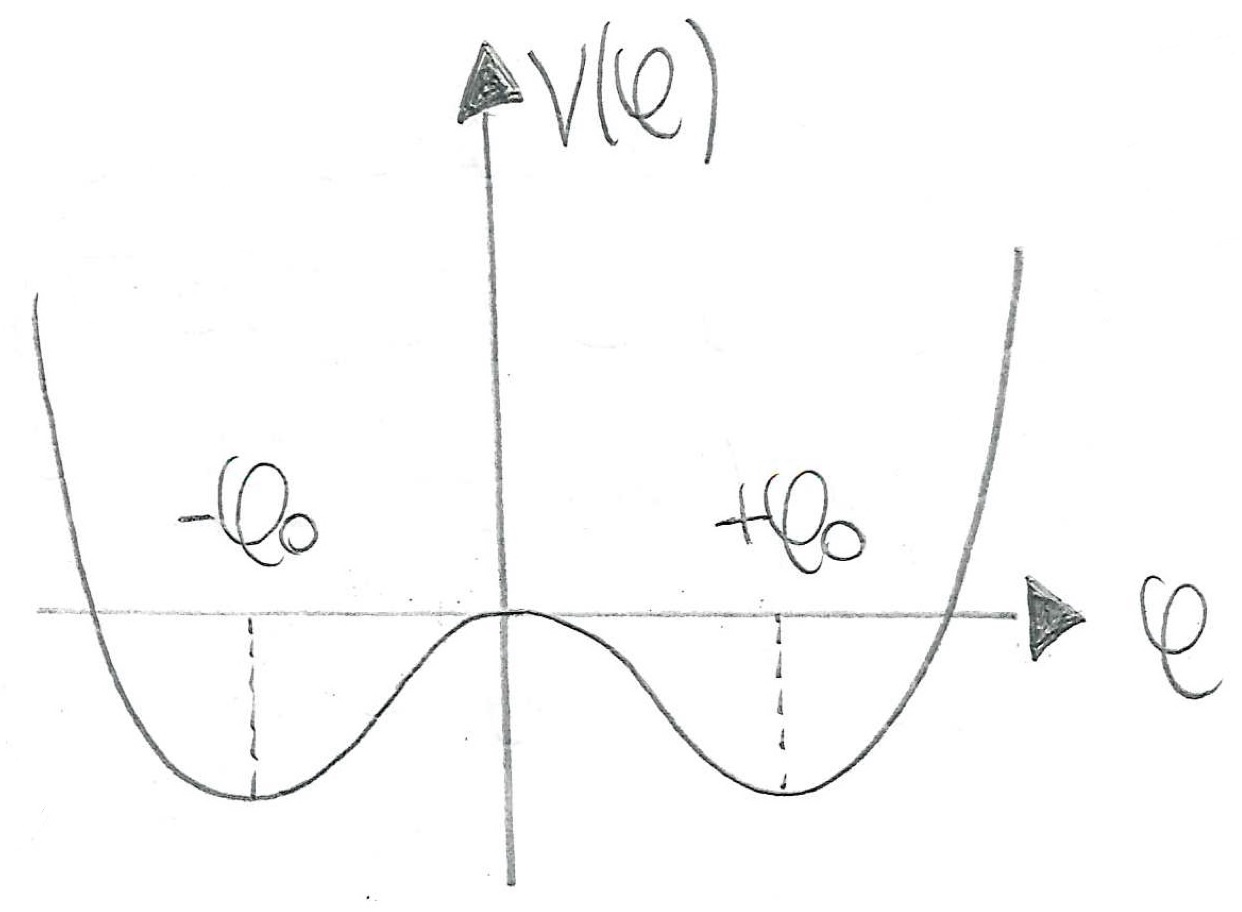
\includegraphics[]{images_ch9/doublewell_potential.jpg}}
Ci sono invece due altre soluzioni, non banali, che annullano la derivata del potenziale, i.e.:
\[
\varphi = \pm\varphi_0 = \pm\frac{\mu}{\sqrt{\lambda}}
\]
Non è difficile convincersi del fatto che queste due soluzioni siano dei minimi e possiamo di conseguenza rappresentare schematicamente il potenziale con cui abbiamo a che fare come fatto a lato.

Abbiamo quindi due stati di vuoto, $\pm \varphi_0$, connessi tra loro per mezzo di una trasformazione di simmetria del tipo $\varphi\rightarrow -\varphi$. Il sistema sceglierà una delle due configurazioni di campo come vero stato di vuoto e \textbf{la simmetria subirà una rottura spontanea}.

È possibile fare, tuttavia, un'intelligente obiezione: \textit{perché mai il sistema sarebbe forzato a compiere una scelta? In fondo siamo interessati ad una situazione di meccanica quantistica in cui potremmo tranquillamente immaginare di avere una sovrapposizione dei due stati degeneri.} Per rispondere al meglio a questa obiezione, consideriamo un esempio in meccanica quantistica.
\marginnote{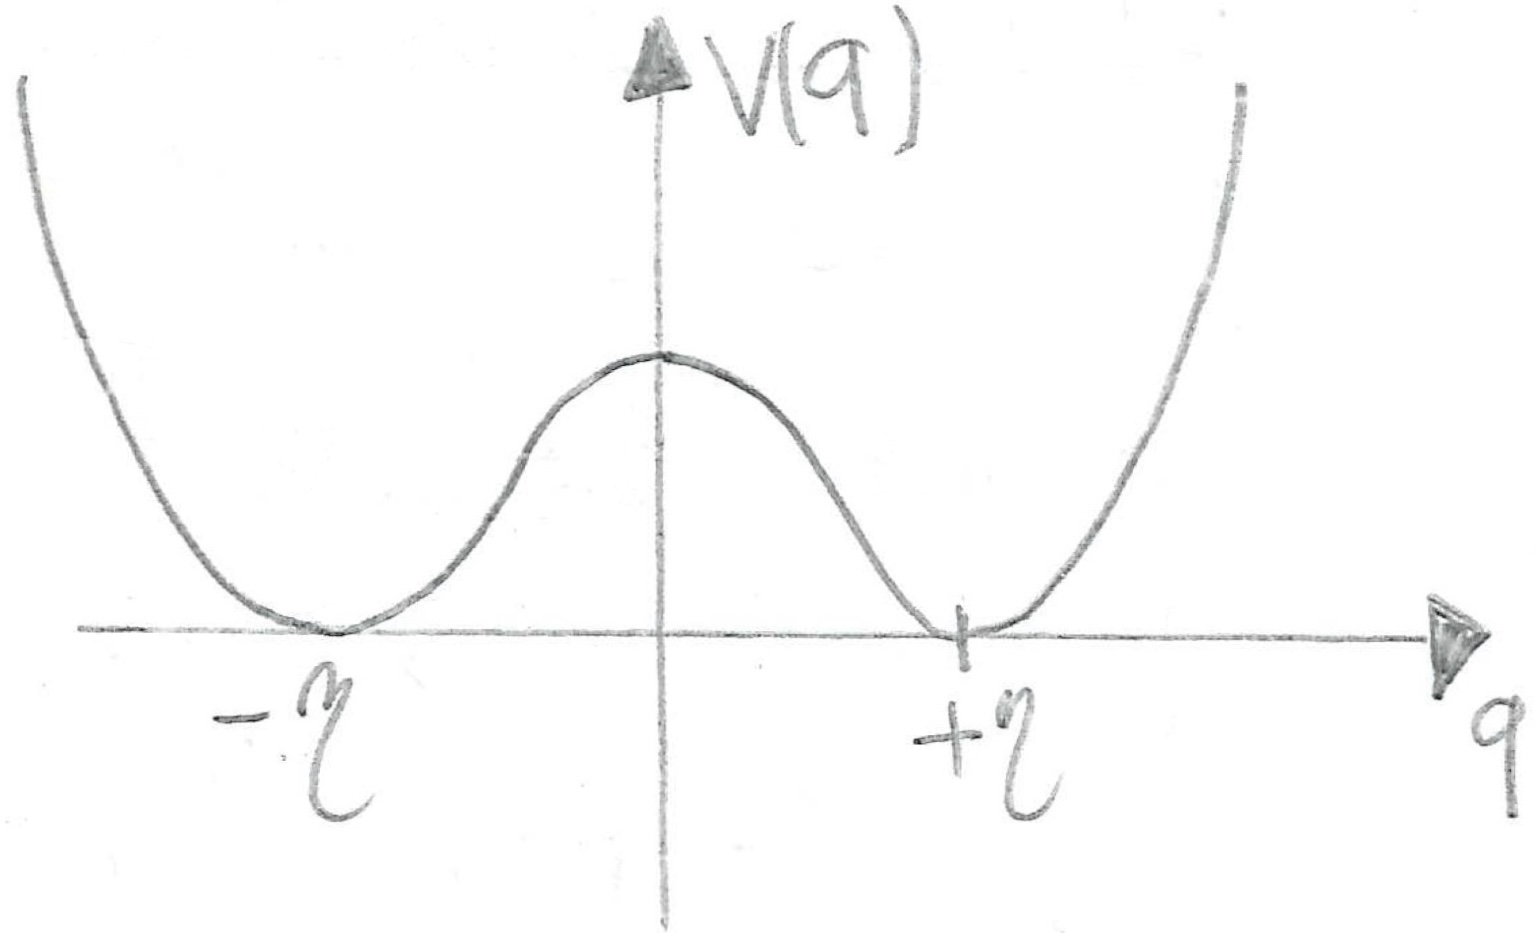
\includegraphics[]{images_ch9/doublewell_potential_example.jpg}}
\begin{example}
    Consideriamo una particella descritta dalla coordinata $q(t)$ con potenziale a doppia buca, con minimi in $\pm\eta$:
    \[
    V(q) = \frac{\lambda^2}{2}\big(q(t)^2-\eta^2\big)^2
    \]
    e la cui Lagrangiana è:
    \[
    \mathscr{L} \frac{1}{2}m\Dot{q}(t)^2 - V(q)
    \]
    simmetrica sotto la trasformazione $q(t)\rightarrow-q(t)$.

    Possiamo risolvere l'equazione di Schrödinger, espandendo il potenziale intorno al minimo in $q=+\eta$ mantenendo solo i termini quadratici nell'espansione, trattando invece come perturbazioni tutti gli ordini superiori, i.e.:
    \[
    V(q) \rightarrow V_{(2)}(q) = 2\eta^2\lambda^2(q-\eta)^2
    \]
    Abbiamo quindi, all'ordine quadratico, un oscillatore armonico con stato di vuoto “$|+\rangle$”.

    Similarmente espandendo attorno a $q=-\eta$ troveremo uno stato di vuoto “$|-\rangle$”.

    Il vero vuoto non è tuttavia nessuno dei due stati, in quanto \textbf{esiste una probabilità di tunneling attraverso la barriera diversa da zero!} In altre parole l'Hamiltoniana non è diagonale nella base $|\pm\rangle$ e si verifica che, alla fine dei conti:
    \[
    \begin{cases}
        \langle+|H|+\rangle = \langle-|H|-\rangle = a \\
        \langle+|H|-\rangle = \langle-|H|+\rangle = b 
    \end{cases}~,\quad b \ll a
    \]
    $b$ è quindi in generale molto piccolo ma non zero, in quanto esponenzialmente soppresso.

    Dopo la diagonalizzazione, gli autostati saranno $|+\rangle\pm|-\rangle$ con autovalori $a\pm b$ e, dipendentemente dal segno di $b$, il vero stato di vuoto sarà 
    \[
    |S\rangle \equiv |+\rangle+|-\rangle \text{ o }|A\rangle \equiv |+\rangle-|-\rangle
    \]
    rispettivamente \textbf{S}immetrico o \textbf{A}nti-simmetrico sotto la trasformazione $q(t)\rightarrow-q(t)$, che trasforma $|+\rangle$ in $|-\rangle$ e viceversa. Ma d'altronde gli stati fisici sono definiti a meno di una fase, quindi alla fine dei conti il vuoto andrà sempre in sé stesso, senza alcun segno di rottura spontanea di simmetria.

    \textbf{In QFT}, la differenza cruciale sta nel fatto che la probabilità di tunneling è zero (\textbf{precisamente zero}, nel limite di volume infinito).

    Per realizzare questo fatto, è utile discretizzare lo spazio e pensare ad un campo quantistico come una collezione di variabili quanto-meccaniche, una per ogni punto nel reticolo. Per far si che il tunneling si verifichi, ognuna di queste particelle deve effettuare il tunneling e per ognuna la probabilità sarà fornita da un esponenziale del tipo $e^{-C}$.

    L'ampiezza totale di tunneling sarà perciò la produttoria delle probabilità individuali in ogni punto del reticolo, che quindi produce un fattore $e^{-CN}$ e, nel limite di spazio continuo, questa ampiezza andrà a zero. 
    
    Tipicamente diciamo che \textbf{una QFT corrisponde alla QM nel limite di infiniti gradi di libertà.}

    Detta in termini diversi: se proviamo a realizzare la transizione $+\varphi_0\rightarrow-\varphi_0$, la configurazione di campo deve cambiare in ciascun punto dello spazio, ma nel limite di volume infinito ciò è impossibile: in QFT i vuoti degeneri sono equivalenti e completamente disconnessi tra loro, quindi può avvenire la rottura spontanea di simmetria.
\end{example}

Ora che abbiamo capito che la SSB è una peculiarità delle teorie quantistiche di campo nel limite di volume infinito, e che ci siamo convinti del fatto che gli stati fondamentali $\pm\varphi_0$ sono completamente disconnessi tra loro, possiamo sceglierne uno come vero stato di vuoto e procedere con la definizione di una nuova teoria sviluppata rispetto ad esso.

In particolare espandiamo il campo attorno allo stato fondamentale $\boxed{\varphi(x) = \varphi_0 + \chi(x)}$ e scriviamo la densità di energia della configurazione di vuoto ricordando che, essendo il campo costante nel tempo ed omogeneo nello spazio, il termine cinetico è nullo:
\begin{align*}
    \mathscr{H}_0 &= -\frac{\mu^2}{2}\varphi_0^2+\frac{\lambda}{4}\varphi_0^4 = -\frac{\mu^4}{2\lambda}+\frac{\mu^4}{4\lambda}\\
    &=-\frac{\mu^4}{4\lambda}
\end{align*}
Possiamo quindi rinormalizzare il punto zero dell'energia a zero, sostanzialmente shiftando il potenziale verso l'alto, ovvero aggiungendo un termine extra alla Lagrangiana pari a $-\mathscr{H}_0$ che non contribuirà alla derivata. Abbiamo quindi, dalla (\ref{eq:lambda_phi^4_lagrangian}):

\begin{equation}
    \mathscr{L} = \frac{1}{2}(\partial_\mu\varphi)(\partial^\mu\varphi) + \frac{\mu^2}{2}\varphi^2  - \frac{\lambda}{4}\varphi^4 + \frac{\mu^4}{4\lambda}
    \label{eq:lambda_phi^4_lagrangian_shifted}
\end{equation}
che con dell'algebra banale si semplifica nella seguente forma:
\begin{equation}
    \boxed{\mathscr{L} = \frac{1}{2}(\partial_\mu\varphi)(\partial^\mu\varphi)   - \frac{\lambda}{4}\big(\varphi^2 - \varphi_0^2 \big)^2}
    \label{eq:lambda_phi^4_lagrangian_shifted_simplif}
\end{equation}
Procediamo ora con l'espansione $\varphi(x) = \varphi_0 + \chi(x)$:
\begin{align*}
    \mathscr{L} &= \frac{1}{2}(\partial_\mu\chi)(\partial^\mu\chi) - \frac{\lambda}{4}\big(\Ccancel[Red]{\varphi_0^2} +\chi^2 +2\varphi_0\chi - \Ccancel[Red]{\varphi_0^2} \big)^2 =\\
    &= \frac{1}{2}(\partial_\mu\chi)(\partial^\mu\chi) - \frac{\lambda}{4}\big(\chi^4 + 4\varphi_0^2\chi^2+ 4\varphi_0\chi^3 \big) =\\
    &= \frac{1}{2}(\partial_\mu\chi)(\partial^\mu\chi) -\lambda\varphi_0^2\chi^2 - \lambda\varphi_0\chi^3 - \frac{\lambda}{4}\chi^4 
\end{align*}

Otteniamo quindi, sostituendo la forma esplicita di $\varphi_0$, la Lagrangiana scalare nella cosiddetta “broken phase”:
\begin{equation}
    \boxed{\mathscr{L}_\chi\equiv \frac{1}{2}(\partial_\mu\chi)(\partial^\mu\chi) - \mu^2\chi^2 -\sqrt{\lambda}\mu\chi^3 - \frac{\lambda}{4}\chi^4 }
    \label{eq:brokenphase_lagrangian}
\end{equation}

Notiamo quindi due cose:
\begin{itemize}
    \item $\mathscr{L}_\chi$ descrive una teoria di campo per un campo massivo scalare $\chi$, in cui sono presenti anche le auto-interazioni di terzo e quart'ordine. \textbf{Tutte le possibili eccitazioni sono massive} e questo non va in contraddizione con il teorema di Goldstone, in quanto la simmetria globale da cui siamo partiti non è continua!

    $\chi$ può essere quantizzato canonicamente introducendo operatori di creazione e distruzione. E di conseguenza non contribuirà al calcolo del VEV del campo $\varphi$, che quindi sarà semplicemente $\varphi_0$, i.e.:
    \[
    \langle0|\varphi(x)|0\rangle = \varphi_0
    \]
    
    $\varphi_0$ \textbf{rappresenta quindi il parametro d'ordine che “misura” la rottura spontanea della simmetria.}

    \item $\mathscr{L}_\chi$ non è invariante sotto $\mathbb{Z}_2$, in quanto presenta un termine cubico in $\chi$, ma ce lo aspettavamo essendo lo stesso vuoto a non essere invariante sotto tale simmetria.

    \textbf{Il residuo della simmetria $\varphi\rightarrow-\varphi$ nella Lagrangiana $\mathscr{L}_\chi$ risiede nella relazione tra la massa di $\chi$ ed i coefficienti dei termini di interazione, detti couplings.} Questo avviene in generale, come nel caso del modello standard con il bosone di Higgs ed i suoi coupling (spoiler).

    Siccome una qualunque Lagrangiana con termini di interazione fino al quartico si può scrivere come:
    \begin{equation}
        \mathscr{L}_\chi\equiv \frac{1}{2}(\partial_\mu\chi)(\partial^\mu\chi) - \frac{m_\chi^2}{2}\chi^2 -\alpha\chi^3 - \frac{\beta}{4}\chi^4 
        \label{eq:general_lagragian_upto_4thorder}
    \end{equation}
    con $m_\chi$, $\alpha$ e $\beta$ arbitrari.

    In presenza di SSB troviamo quindi la seguente relazione tra la massa di $\chi$ ed i coupling di interazione:
    \begin{equation}
        m_\chi^2 = 2\mu^2~,\quad
        \alpha = \sqrt{\lambda}\mu~,\quad
        \beta = {\lambda}
        \label{eq:mass_coupling_relations}
    \end{equation}
\end{itemize}

\subsection{SSB della simmetria U(1)}

Consideriamo ora il caso di un campo scalare complesso $\varphi \equiv \frac{1}{\sqrt{2}}(\varphi_1+i\varphi_2)$ descritto dalla Lagrangiana:

\begin{equation}
    \boxed{\mathscr{L} = (\partial_\mu\varphi^\ast)(\partial^\mu\varphi) - m^2\varphi^\ast\varphi - \lambda(\varphi^\ast\varphi)^2 - C}
    \label{eq:charged_scalar_lagrangian}
\end{equation}
dove $C$ è una costante arbitraria che serve a dare un offset al potenziale, allo scopo di rinormalizzare il punto zero dell'energia.

Eventualmente, possiamo riscrivere questa Lagrangiana esplicitando le componenti reali del campo $\varphi$, i.e.:
\[
\mathscr{L} = \frac{1}{2}\sum_{i=1}^2(\partial_\mu\varphi_i)(\partial^\mu\varphi_i) - \frac{m^2}{2}\sum_{i=1}^2\varphi_i^2 - \frac{\lambda}{4}\bigg(\sum_{i=1}^2\varphi_i^2\bigg)^2
\]

È evidente il fatto che la (\ref{eq:charged_scalar_lagrangian}) possieda una simmetria globale $\textrm{U}(1)$, i.e. $\varphi'(x)=e^{i\alpha}\varphi(x)$, mentre in termini delle componenti $\varphi_{1,2}$ la simmetria è di tipo $\textrm{SO}(2)$, i.e. una rotazione 2D nello spazio reale dei campi.

Come nel caso precedente, consideriamo l'energia del campo 
:
\begin{align*}
    &H=\int_{}d^3\Vec{x}\bigg[ (\partial_t\varphi^\ast)(\partial_t\varphi) + (\partial_i\varphi^\ast)(\partial^i\varphi) + V(\varphi, \varphi^\ast)\bigg]\\
    &V(\varphi, \varphi^\ast) = m^2\varphi^\ast\varphi + \lambda(\varphi^\ast\varphi)^2 + C
\end{align*}
\begin{itemize}
\marginnote{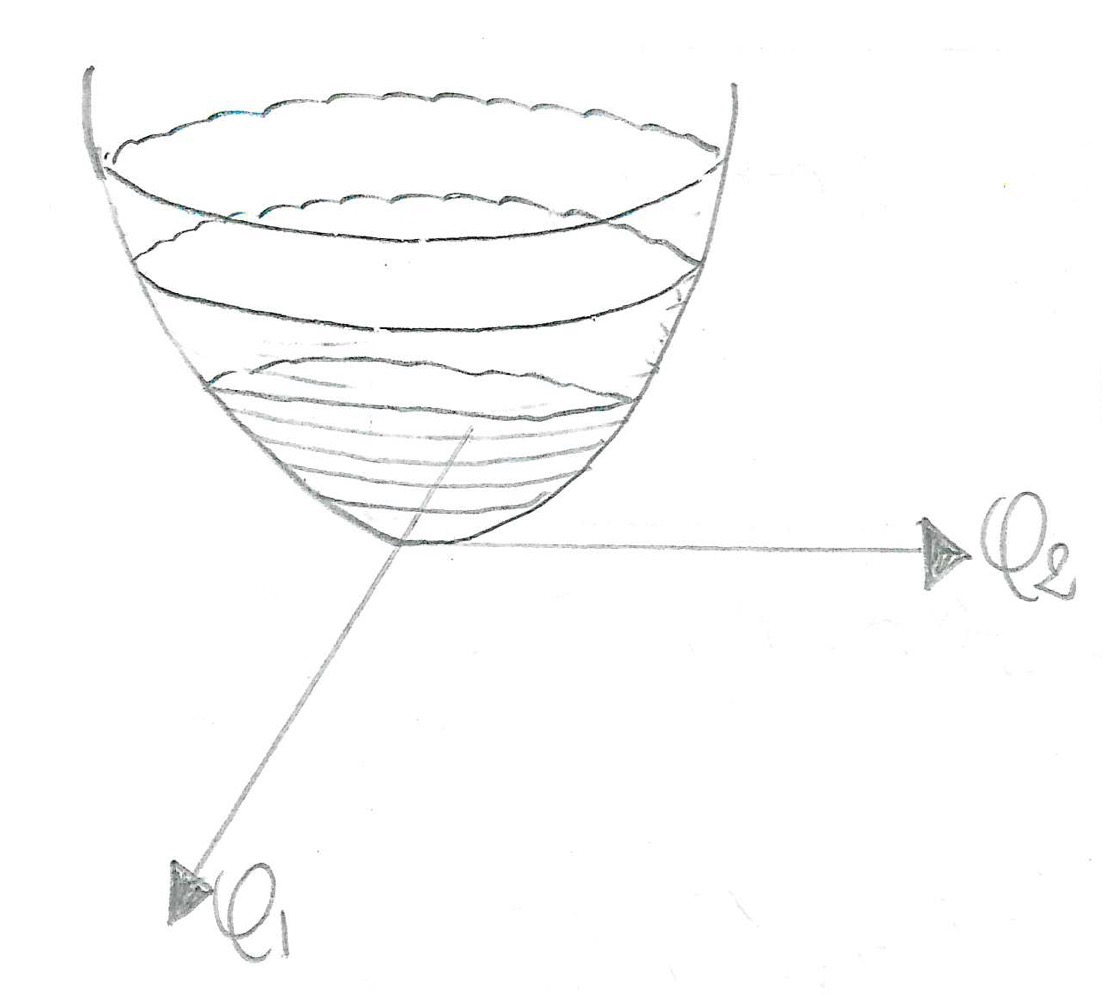
\includegraphics[]{images_ch9/U1_potential.jpg}}
    \item Quando $m^2\geq 0$ la situazione è noiosa, il potenziale ha la struttura riportata a lato, con minimo in $\varphi_1=\varphi_2=0$ e la simmetria non è rotta.

    \item Il caso interessante è nuovamente quello in cui $m^2=-\mu^2<0$, con $\mu^2>0$. Se andiamo a minimizzare il potenziale, innanzitutto notiamo che questo dipende dal solo modulo $|\varphi|$, i.e.:
    \[
    V(|\varphi|) = -\mu^2|\varphi| + \lambda(|\varphi|)^2 + C
    \]
    Non è a questo punto difficile convincersi del fatto che:
    \begin{align*}
        &\frac{\partial V}{\partial |\varphi|} = 0 \Rightarrow |\overline{\varphi}|^2 = \frac{\mu^2}{2\lambda}\\
        &\frac{\partial^2 V}{\partial |\varphi|^2}\bigg|_{|\overline{\varphi}|^2} = 4\mu^2>0 \Rightarrow \overline{\varphi} \text{ è minimo}
    \end{align*}
    Abbiamo quindi un insieme di minimi degeneri, tutti legati tra loro da una trasformazione di $\textrm{U}(1)$, i.e.
    \[
    \boxed{\overline{\varphi} = e^{i\alpha}\frac{\varphi_0}{\sqrt{2}}~,\quad \varphi_0 = \frac{\mu}{\sqrt{\lambda}}}
    \]
    Scegliamo quindi $C$ in modo tale che il potenziale si azzeri nel minimo, e per determinare il valore necessario prendiamo:
    \marginnote{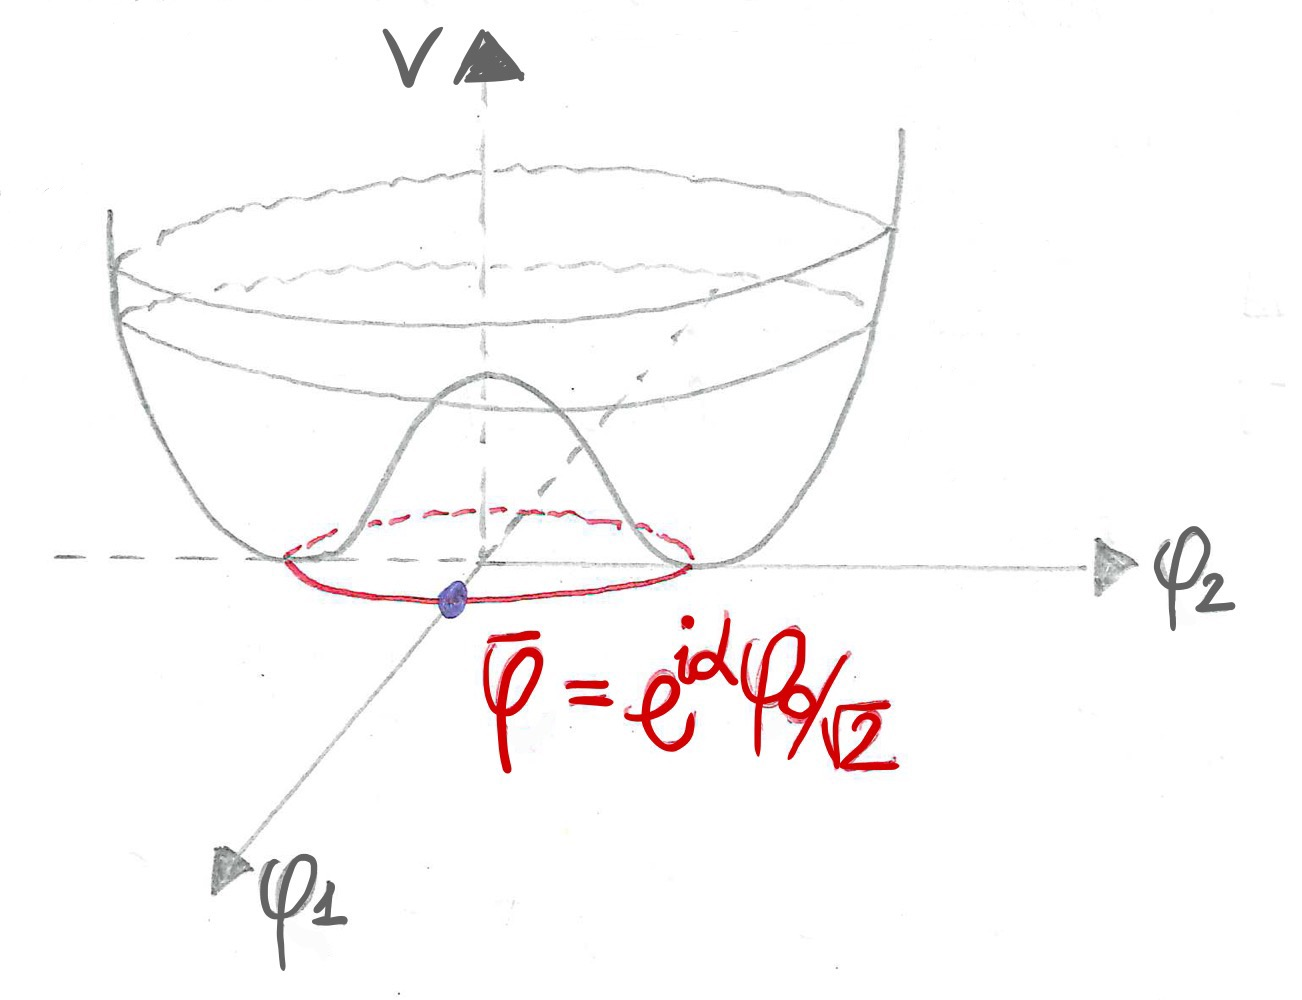
\includegraphics[]{images_ch9/U1_potential_brokensymm.jpg}}
    \[
    V(|\overline{\varphi}| = \nicefrac{\mu}{\sqrt{\lambda}}) = 0 \Rightarrow \boxed{C= \frac{\mu^4}{4\lambda}}
    \]
    La situazione schematica nello spazio dei campi reali è quindi quella riportata al lato: un insieme di minimi degeneri identificati dal cerchio rosso. Il sistema sceglie spontaneamente uno di questi minimi come stato di vuoto: abbiamo una rottura spontanea di simmetria!
\end{itemize}

Mettiamoci quindi nella situazione di SSB e facciamo noi la scelta al posto del sistema. Consideriamo per esempio
\[
\Bar\varphi_1 \equiv \varphi_0 ~,~\Bar\varphi_2 = 0 \Rightarrow \boxed{\overline{\varphi} = \frac{\varphi_0}{\sqrt{2}}}
\]
Espandiamo a questo punto intorno a questo vuoto, definendo i \textbf{campi shiftati}:
\begin{equation}
    \boxed{
    \begin{aligned}
        &\varphi_1(x)\equiv \varphi_0 + \chi(x) \\
        &\varphi_2(x)\equiv \theta(x)
    \end{aligned}}
    \label{eq:shifted fields}
\end{equation}


Da cui ricaviamo il \textbf{parametro d'ordine} $\langle0|\varphi_1|0\rangle= \varphi_0\neq0$.

Andiamo quindi a riscrivere la Lagrangiana in termini di $\chi(x)$ e $\theta(x)$:
\begin{itemize}
    \item[\blacksquare] \textbf{Termini cinetici} 

    Questa è la parte facile, $\varphi_0$ è costante, quindi si tratta semplicemente di sostituire (partendo dalla Lagrangiana espressa nelle componenti reali) $\varphi_1$ e $\varphi_2$ con  $\chi$ e $\theta$ rispettivamente. Otteniamo quindi:
    \begin{equation}
        \mathscr{L}_\text{kin} = \frac{1}{2}(\partial_\mu\chi)(\partial^\mu\chi)+\frac{1}{2}(\partial_\mu\theta)(\partial^\mu\theta)
        \label{eq:kinetic_terms_U1_SSB}
    \end{equation}
    \item[\blacksquare] \textbf{Potenziale}

    Qui la questione è un po' più noiosa, bisogna farsi i conti \textbf{[Lez. 35 pag 37]}, ma la sostanza è che gli ordini $0$ e $1$ (lineare) in entrambi campi si annullano, così come l'ordine $2$ (quadratico) nel campo $\theta$. 

    \textbf{Sopravvivono quindi solo l'ordine quadratico in $\chi$ e le interazioni cubiche e quartiche:}
    \begin{equation}
        V(\chi, \theta) = \mu^2\chi^2 + \frac{\lambda}{4}\big(\chi^4 + \theta^4 + 4\chi^3\varphi_0 +2\chi^2\theta^2 \big)
        \label{eq:potential_terms_U1_SSB}
    \end{equation}
\end{itemize}
Troviamo quindi in definitiva la densità di Lagrangiana nella broken phase ($\mathscr{L} = \mathscr{L}_\text{kin} - V$) che cercavamo, composta da una parte quadratica (i primi tre termini) e dalle interazioni (la parte proporzionale a $\nicefrac{\lambda}{4}$), i.e.:
\begin{equation}
    \boxed{\begin{aligned}
        \mathscr{L}_{BP} =& \frac{1}{2}(\partial_\mu\chi)(\partial^\mu\chi) -\mu^2\chi^2 +\frac{1}{2}(\partial_\mu\theta)(\partial^\mu\theta) \\
        &-\frac{\lambda}{4}\big(\chi^4 + \theta^4 + 4\chi^3\varphi_0 +2\chi^2\theta^2 \big)
    \end{aligned}}
    \label{eq:brokenphase_lagrangian_U1_SSB}
\end{equation}
Ci accorgiamo immediatamente del fatto che \textbf{il campo $\chi$ è un campo massivo}, con massa $m_\chi = \sqrt{2}\mu$\footnote{Per quanto segue dalla (\ref{eq:general_lagragian_upto_4thorder}).}, mentre il campo $\theta$ è massless, i.e.: \textbf{$\theta(x)$ è il campo di Goldstone!}

\begin{exercise}
    Proviamo a connettere quanto appena visto con la dimostrazione formale del teorema di Goldstone.
    Innanzitutto discutiamo la proposizione \ref{prop:nonvanishing_vm_implication}, che ci dice che per almeno una “$A$” ed una “$m$”, deve valere:
    \begin{equation}
        \langle 0|\big[Q_A, O_m(x)\big]|0\rangle \neq 0 = -(T^A)_{mn}\langle 0|O_n(x)|0\rangle
        \label{eq:commutator_VEV}
    \end{equation}
    dove l'espressione esplicita in termini di $T^A$ è stata ricavata nella rispettiva dimostrazione.

    \begin{itemize}
    \item \textbf{Consideriamo la Lagrangiana nella base dei campi reali} $\varphi_{1,2}$, i.e.:
    \[
    \mathscr{L} = \frac{1}{2}\sum_{i=1}^2(\partial_\mu\varphi_i)(\partial^\mu\varphi_i) - \frac{m^2}{2}\sum_{i=1}^2\varphi_i^2 - \frac{\lambda}{2}\bigg(\sum_{i=1}^2\varphi_i^2\bigg)^2
    \]
    Abbiamo già sottolineato che in questo caso la simmetria globale è realizzata dalle rotazioni di $\textrm{SO}(2)$, con il vettore $\Vec{\varphi} \equiv \begin{pmatrix}\varphi_1\\ \varphi_2\end{pmatrix}$ che trasforma secondo la rappresentazione fondamentale, vale a dire:
    \[
    \begin{pmatrix}
    \varphi_1\\ 
    \varphi_2
    \end{pmatrix} \xrightarrow{\textrm{SO}(2)}
    R(\phi)\begin{pmatrix}
    \varphi_1\\ 
    \varphi_2
    \end{pmatrix} =
    e^{-i\phi T} \begin{pmatrix}
    \varphi_1\\ 
    \varphi_2
    \end{pmatrix}\simeq \big(\mathbb 1 - i\phi T\big)\begin{pmatrix}
    \varphi_1\\ 
    \varphi_2
    \end{pmatrix}
    \]
    Essendo il generatore della simmetria esprimibile con la matrice $T \equiv \begin{pmatrix}
    0&-i\\ 
    i&0
    \end{pmatrix}$, la trasformazione esplicita assume la forma:
    \[
    \begin{pmatrix}
    \varphi_1\\ 
    \varphi_2
    \end{pmatrix}\xrightarrow{\textrm{SO}(2)}
    \begin{pmatrix}
    \varphi_1 - \phi\varphi_2\\ 
    \varphi_2 + \phi\varphi_1
    \end{pmatrix} \Rightarrow 
    \boxed{\begin{cases}
        \delta\varphi_1 \equiv -\phi\varphi_2\\
        \delta\varphi_2 \equiv \phi\varphi_1
    \end{cases}}
    \]
    \item \textbf{Possiamo quindi ricavare la corrente di Noether} $j^\mu$:
    \[
    j^\mu = \frac{\partial\mathscr{L}}{\partial\big(\partial_\mu\varphi_1\big)}\frac{\delta\varphi_1
    }{\delta\phi} +\frac{\partial\mathscr{L}}{\partial\big(\partial_\mu\varphi_2\big)}\frac{\delta\varphi_2
    }{\delta\phi}= \big(\partial^\mu\varphi_1\big)(-\varphi_2) + \big(\partial^\mu\varphi_2\big)\varphi_1
    \]
    A questa corrente corrisponde una carica conservata, l'integrale spaziale della componente temporale di $j^\mu$. Le riportiamo insieme:
    \begin{equation}
        \boxed{
        \begin{aligned}
        &j^\mu(x) \equiv
        \big(\partial^\mu\varphi_2(x)\big)\varphi_1(x) -\big(\partial^\mu\varphi_1(x)\big)\varphi_2(x)\\
        &Q \equiv \int_{}d^3\Vec{x}\big[\big(\partial_t\varphi_2\big)\varphi_1 - \big(\partial_t\varphi_1\big)\varphi_2\big]
        \end{aligned}}
        \label{eq:U1_noether_current_and_charge}
    \end{equation}

    \item \textbf{Calcoliamo ora esplicitamente il commutatore} $\big[Q_A, O_m\big]$, nel caso di una singola carica conservata e con $O_m= \Vec{\varphi}$. Con riferimento alla (\ref{eq:commutator_VEV}), e conoscendo la struttura del generatore $T$, troviamo:
    \[
    \big[Q, \Vec{\varphi}\big] = -
    \begin{pmatrix}
    0&-i\\ 
    i&0
    \end{pmatrix}
    \begin{pmatrix}
    \varphi_1\\ 
    \varphi_2
    \end{pmatrix} = -\begin{pmatrix}
    -i\varphi_2\\ 
    i\varphi_1
    \end{pmatrix}
    \]
    ovvero:
    \begin{equation}
        \boxed{\big[Q, \Vec{\varphi}_1\big] = i\varphi_2~,\quad \big[Q, \Vec{\varphi}_2\big] = -i\varphi_1}
        \label{eq:commutator_explicit_U1}
    \end{equation}
    
    \item \textbf{In presenza di rottura spontanea di simmetria}, il parametro d'ordine $\langle0|\varphi_1|0\rangle = \varphi_0\neq 0$, ma allora dalla (\ref{eq:commutator_explicit_U1}):
    \[
    \boxed{\langle0|\big[Q, \Vec{\varphi}_2\big]|0\rangle = -i\langle0|\varphi_1|0\rangle = -i\varphi_0\neq 0}
    \]
    Ecco la proposizione “al lavoro”: quando il parametro d'ordine della teoria, $\varphi_0$, è diverso da zero, anche il VEV del commutatore $\big[Q, \Vec{\varphi}_2\big]$ è diverso da zero, e questo è esattamente l'oggetto che entra nella dimostrazione del teorema di Goldstone da noi delineata in precedenza.
    \end{itemize}

    Per completezza verifichiamo anche la validità della condizione finale ricavata nella dimostrazione del teorema, ovvero l'equazione (\ref{eq:rho_explicit_form}):
    \[
    {\rho}_{A,n}(\mu^2) = - \delta(\mu^2)\big(T^A\big)_{nm}\langle0|O_m(x)|0\rangle
    \]
    che nel nostro caso diventa:
    \begin{equation}
        \boxed{\rho_2(\mu^2) = -\delta(\mu^2)i\varphi_0}
        \label{eq:rho_explicit_form_U1}
    \end{equation}

    Allo stesso modo possiamo riscrivere la struttura di $\rho^\mu$, partendo dalla (\ref{eq:rho_structure}), ottenendo:
    \begin{equation}
        \begin{aligned}
            \frac{1}{(2\pi)^3}\rho^\mu_{A,n}(p) &= \frac{1}{(2\pi)^3}p^\mu (-i\varphi_0)\delta(p^2)\Theta(p^0) =\\ &=  \sum_N\langle 0|j^\mu(0) |N\rangle\langle N| \varphi_2(0)|0\rangle \delta^{(4)}(p-p_N)
        \end{aligned}
        \label{eq:rho_structure_U1}
    \end{equation}
    Ricordiamo ora il fatto che $\sum_N$ è una somma “generalizzata”, quindi include anche un integrale sollo spazio dell'impulso. Questo, combinato con il fatto che dalla somma abbiamo solo il contributo di una particella (connessa al campo $\varphi_2$), restituisce la seguente espressione per il RHS:
    \[
    \textbf{RHS} = \int_{}\frac{d^3\Vec{k}}{(2\pi)^32k^0}\langle 0|j^\mu(0) |\Vec{k}\rangle\langle \Vec{k}| \varphi_2(0)|0\rangle \delta(p-k)
    \]
    con $k^0=|\Vec{k}|$ in quanto lo stato $|N\rangle$ deve rappresentare una particella massless.

    Possiamo quindi svolgere il calcolo esplicito, introducendo i campi shiftati (\ref{eq:shifted fields}). Piuttosto banalmente si trova per la corrente:
    \[
    j^\mu \equiv \big(\partial^\mu\theta\big)\varphi_0 + \big[\chi \big(\partial^\mu\theta\big) -\big(\partial^\mu\chi\big)\theta\big]
    \]
    Lavoriamo ora sull'integranda $\langle 0|j^\mu(0) |k\rangle\langle k| \varphi_2(0)|0\rangle $, in particolare notando il fatto che, essendo necessariamente il termine relativo a $\varphi_2$ non nullo, lo stato $|k\rangle$ deve essere creato dal vuoto da $\theta$. Questo comporta quindi che nel bra-ket relativo alla corrente, solo il termine $(\partial^\mu\theta)\varphi_0$ contribuisce! In formule:
    \[
    \langle 0|j^\mu(0) |k\rangle\langle k| \varphi_2(0)|0\rangle = \langle 0|(\partial^\mu\theta)\varphi_0 |\Vec{k}\rangle\langle \Vec{k}| \theta(0)|0\rangle
    \]
    A questo punto scriviamo $\theta(x)$ in funzione degli operatori di creazione e distruzione:
    \begin{align*}
        &\theta(x) = \int_{}\frac{d^3\Vec{p}}{(2\pi)^3\sqrt{2p^0}} \Big(a(\Vec{p})e^{-ip\cdot x} +a^\dagger(\Vec{p})e^{ip\cdot x}\Big)\\
        &\big[a(\Vec{p}), a^\dagger(\Vec{k})\big] = (2\pi)^3\delta(\Vec{p} -\Vec{k}) \\
        &|\Vec{p}\rangle = \sqrt{2E_p}a^\dagger(\Vec{p})|0\rangle
    \end{align*}

    Abbiamo quindi:
    \begin{align*}
        \langle \Vec{k}| \theta(x)|0\rangle &=\sqrt{2E_k}\langle 0|a(\Vec{k}) \theta(x)|0\rangle =\\
        &=\int_{}\frac{d^3\Vec{p}}{(2\pi)^3\sqrt{2p^0}}(2\pi)^3\delta(\Vec{p} -\Vec{k})\sqrt{2E_k}e^{ip\cdot x}\\
        &=e^{ik\cdot x}
    \end{align*}
    Ma allora: \( \boxed{\langle k| \theta(0)|0\rangle = 1}\) !

    D'altro canto l'azione di $\partial^\mu$ su $\theta(x)$ porta giù un fattore $(\pm ip^\mu)$ dall'esponenziale, quindi senza troppa difficoltà possiamo scoprire che:
    \[\langle 0|\big(\partial^\mu\theta(x)\big)\varphi_0|\Vec{k}\rangle = (-ik^\mu)\varphi_0e^{-ik\cdot x}\]
    Ergo $\boxed{\langle 0|\big(\partial^\mu\theta(0)\big)\varphi_0|\Vec{k}\rangle = (-i\varphi_0)k^\mu}$ !

    Se ora torniamo al RHS da cui siamo partiti, sostituiamo quanto appena appreso, separiamo la delta di Dirac ed integriamo su $\Vec{k}$, otteniamo:
    \begin{align*}
        \textbf{RHS} &= \int_{}\frac{d^3\Vec{k}}{(2\pi)^32k^0}(-i\varphi_0)k^\mu \delta^{(1)}(p^0-|\Vec{k}|) \delta^{(3)}(\Vec{p}-\Vec{k}) = \\
        &= \frac{(-i\varphi_0)p^\mu}{(2\pi)^32p^0} \delta^{(1)}(p^0-|\Vec{p}|)
    \end{align*}
    Abbiamo sostanzialmente finito, ci basta ricordare l'identità:
    \[
    \delta(p^2) = \delta\big((p^0)^2-|\Vec{p}|^2\big) =\frac{1}{2p^0}\delta(p^0-|\Vec{p}|) + \frac{1}{2p^0}\delta(p^0+|\Vec{p}|)
    \]
    da cui estraiamo il primo termine moltiplicandola per una theta di Heaviside, i.e. $\delta(p^2)\Theta(p^0) = \frac{1}{2p^0}\delta(p^0-|\Vec{p}|)$. 

    Troviamo quindi in definitiva:
    \begin{equation}
        \boxed{\textbf{RHS} = \frac{1}{(2\pi)^3} (-i\varphi_0)p^\mu\delta(p^2)\Theta(p^0)}
        \label{eq:RHS_rhomu}
    \end{equation}
    perfettamente in accordo con il LHS della (\ref{eq:rho_structure_U1})
\end{exercise}

\section{Realizzazione non Lineare della SSB di U(1)}
\label{sec:non_linear_U1_SSB}
Discutiamo ora una differente parametrizzazione, in grado di rendere più evidente la fisica dietro il teorema di Goldstone. 

Consideriamo nuovamente la teoria descritta dalla (\ref{eq:charged_scalar_lagrangian}), invariante sotto $\textrm{U}(1)$:
\[
\mathscr{L} = (\partial_\mu\varphi^\ast)(\partial^\mu\varphi) +\mu^2\varphi^\ast\varphi - \lambda(\varphi^\ast\varphi)^2 - \frac{\mu^4}{4\lambda}
\]

Consideriamo nuovamente come vuoto:
\[
\langle 0|\varphi(x)|0\rangle = \frac{\varphi_0}{\sqrt{2}}
\]
ma questa volta invece di adottare una parametrizzazione cartesiana per i campi shiftati, che produrrebbe
\[
\varphi(x) = \frac{\varphi_0}{\sqrt{2}} + \frac{1}{\sqrt{2}}\big[\chi(x) + i \theta(x)\big]
\]
utilizziamo una decomposizione polare, scrivendo
\begin{equation}
    \boxed{\varphi(x) \equiv \frac{1}{\sqrt{2}} \big[\varphi_0 + \sigma(x)\big]\exp[\frac{i\pi(x)}{f_\pi}]}
    \label{eq:shifted_field_polar}
\end{equation}
dove $\sigma(x)$ e $\pi(x)$ sono campi scalari reali, denominati rispettivamente campo “\textit{radiale}” ed “\textit{angolare}”.

“$f_\pi$”, invece, è un parametro la cui dimensione di massa rende l'argomento dell'esponenziale adimensionale.

Andiamo quindi ad analizzare la Lagrangiana nella broken phase in questa particolare parametrizzazione: 
\begin{itemize}
    \item[\blacklozenge] \textbf{Termine cinetico}

    Con le giuste accortezze, partendo dal termine $(\partial_\mu\varphi^\ast)(\partial^\mu\varphi)$, si arriva a 
    \begin{equation}
        \mathscr{L}_\text{kin} = \frac{1}{2}(\partial_\mu\sigma)(\partial^\mu\sigma) +\frac{\varphi_0^2}{2f_\pi^2}(\partial_\mu\pi)(\partial^\mu\pi) + \frac{1}{2f_\pi^2}(2\varphi_0\sigma + \sigma^2)(\partial_\mu\pi)(\partial^\mu\pi)
        \label{eq:kinetic_lagrangian_nonlinear}
    \end{equation}
    Se poi fissiamo $\boxed{f_\pi = \varphi_0}$ otteniamo il termine cinetico di $\pi$ canonicamente normalizzato.
    
    \item[\blacklozenge] \textbf{Termine di potenziale}
    
    Per quanto riguarda il potenziale si tratta di svolgere della noiosa algebra, durante la quale bisogna ricordare che $\varphi_0^2 = \frac{\mu^2}{\lambda}$. Alla fine dei conti si ottiene:
    \begin{equation}
        V(\sigma, \pi) = \mu^2\sigma^2 + \lambda\varphi_0\sigma^3 + \frac{\lambda}{4}\sigma^4
        \label{eq:potential_nonlinear}
    \end{equation}
\end{itemize}
Raccogliendo quanto appena appreso, possiamo scrivere la Lagrangiana totale nella broken phase, $\mathscr{L}_\text{kin} - V$:

\begin{equation}
    \boxed{\begin{aligned}
        \mathscr{L}_{BP} =& \frac{1}{2}(\partial_\mu\sigma)(\partial^\mu\sigma) - \mu^2\sigma^2 +\frac{1}{2}(\partial_\mu\pi)(\partial^\mu\pi) \\
        &+ \frac{1}{2\varphi_0^2}(2\varphi_0\sigma + \sigma^2)(\partial_\mu\pi)(\partial^\mu\pi) - \lambda\varphi_0\sigma^3 - \frac{\lambda}{4}\sigma^4
    \end{aligned}}
    \label{eq:broken_phase_lagrangian_nonlinear}
\end{equation}
In questo caso il campo massivo è $\sigma(x)$, e presenta auto-interazioni cubiche e quartiche. 

D'altro canto il campo di Goldstone è $\pi(x)$, essendo questo un campo massless.
\marginnote{
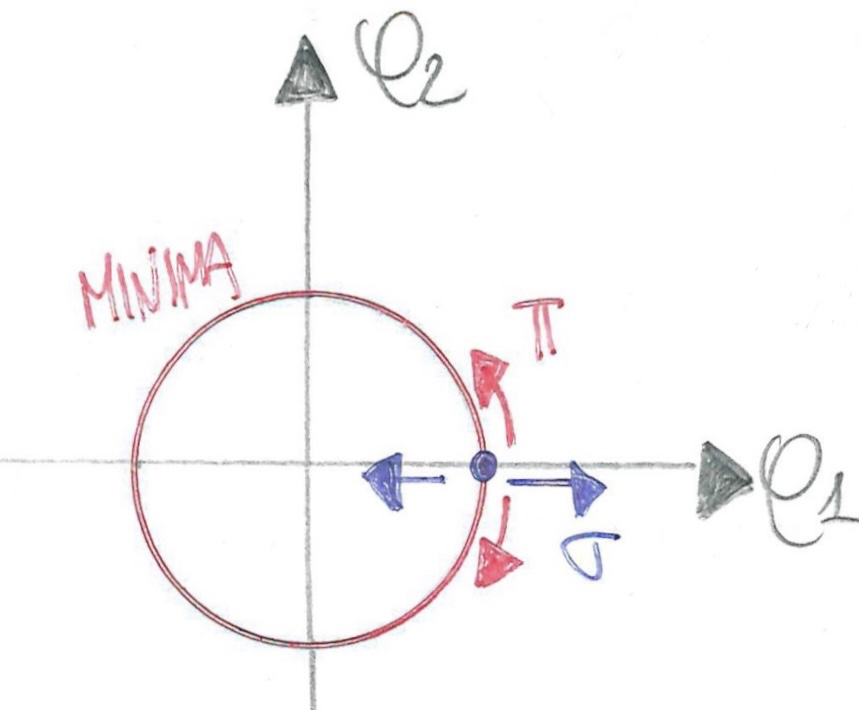
\includegraphics[]{images_ch9/intuitive_interpr_above.jpg} Potenziale visto “da sopra”.}

Fin qui tutto come prima, ma ora possiamo dare due interpretazioni alla non-massività di $\pi$:
\begin{enumerate}
    \item[\textbf{i)}] \textbf{Interpretazione intuitiva dal punto di vista grafico.}
    
    \textbf{$\pi(x)$ descrive le fluttuazioni angolari}, lungo questa direzione (ovvero la direzione parallela al piano, intuibile dalla figura a lato in cui il potenziale è visto dall'alto), detta “\textit{direzione flat}” non c'è alcun pontenziale, in quanto ci stiamo muovendo sulla circonferenza dei minimi del potenziale, che abbiamo off-settato a zero. Dall'assenza di potenziale segue la non-massività.
    \marginnote{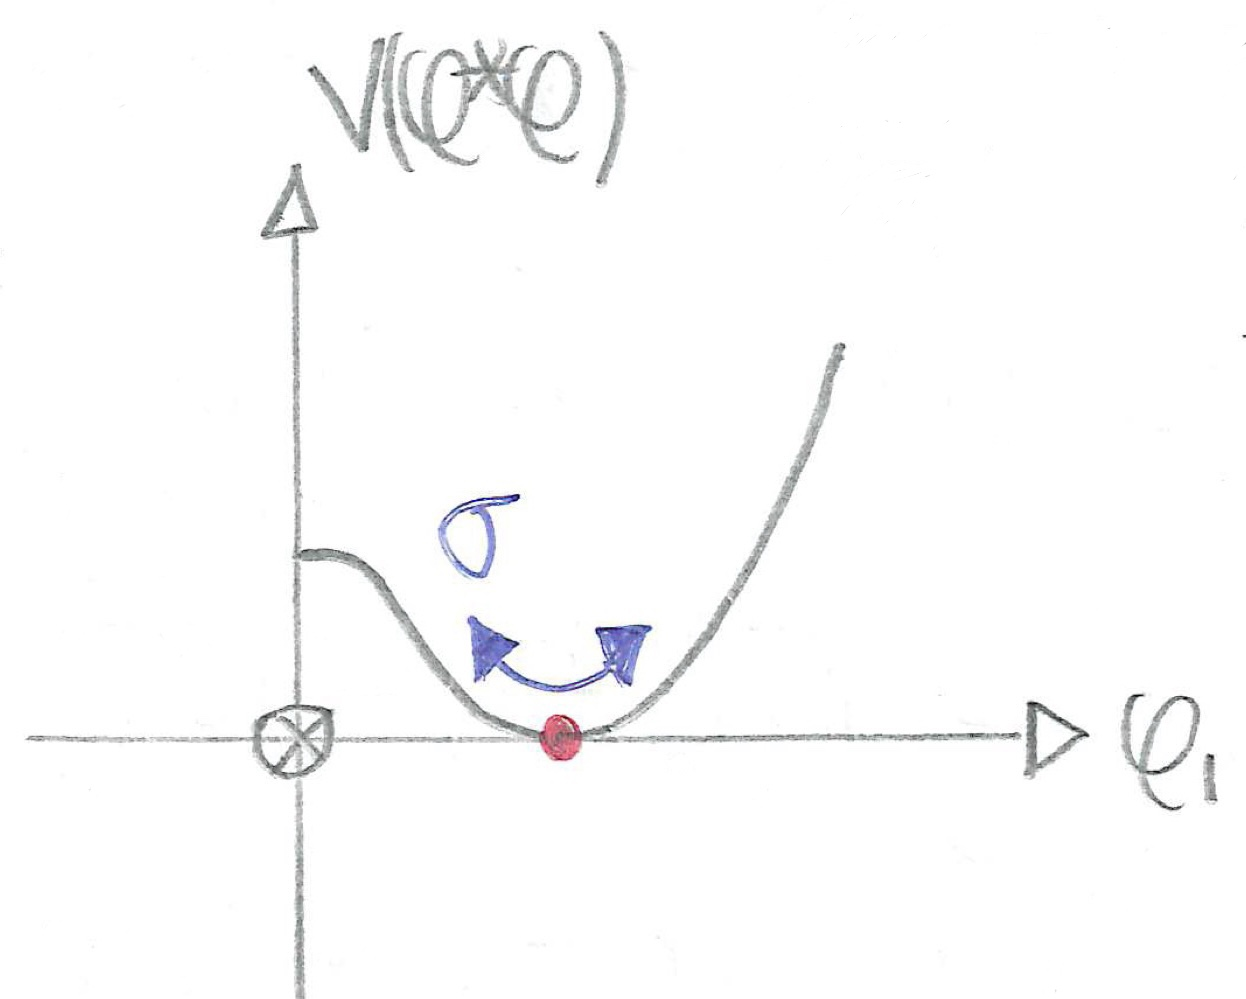
\includegraphics[]{images_ch9/intuitive_interpr_section.jpg} Potenziale visto in sezione, con l'asse di $\varphi_2$ uscente dal foglio/schermo.}

    D'altro canto \textbf{$\sigma(x)$ descrive le fluttuazioni radiali} e lungo questa direzione c'è potenziale, come si intuisce dalla figura in cui è rappresentato il potenziale visto in sezione. Questo fornisce quindi a $\sigma$ un termine di massa!
    
    \item[\textbf{ii)}] \textbf{Interpretazione in termini di realizzazione non lineare della simmetria.}

    Torniamo alla Lagrangiana nella broken phase (\ref{eq:broken_phase_lagrangian_nonlinear}). Questa possiede una simmetria detta “\textbf{simmetria di shift}”, ovvero è invariante sotto una trasformazione che produca uno shift dei campi di un termine costante, e.g. $\pi(x)\rightarrow \pi(x) + cost.$, la verifica è piuttosto ovvia, in quanto $\pi(x)$ figura nella Lagrangiana solo sotto derivata.

    Trasformazioni di questo tipo corrispondono precisamente ad un movimento nella direzione flat.

    Inoltre, se torniamo alla definizione (\ref{eq:shifted_field_polar}), notiamo come ad uno shift di $\pi(x)$ corrisponda una rotazione di $\varphi(x)$ per mezzo di una fase. Questo significa che \textbf{la simmetria originale} $\varphi\rightarrow e^{i\alpha}\varphi$ \textbf{è ancora presente nella broken phase ma si realizza in maniera non lineare, sotto forma della simmetria di shift del campo di Goldstone.} Inoltre è precisamente questa simmetria di shift impedisce la presenza del termine di massa per il campo di Goldstone!\footnote{Perché, come abbiamo notato precedentemente, alla simmetria di shift corrisponde uno spostamento sulla circonferenza dei minimi, con potenziale nullo.}

    In sintesi, \textit{la differenza tra la broken e l'unbroken phase della Lagrangiana corrisponde ad una differente realizzazione della simmetria:}
    \begin{itemize}
        \item \textbf{Unbroken Phase.}
        \begin{itemize}
            \item Simmetria realizzata linearmente rispetto ai campi dinamici: $\varphi(x) \rightarrow e^{i\alpha}\varphi(x)$ ;
            \item Vuoto unico;
            \item Simmetria realizzata sullo spettro della teoria:
            \begin{align*}
                &Q|0\rangle = |0\rangle ~,\quad |M,\Vec{p}\rangle\otimes|q\rangle = |M,\Vec{p},q\rangle\\
                &Q|q\rangle = |q\rangle
            \end{align*}
        \end{itemize}
        \item \textbf{Broken Phase.}
        \begin{itemize}
            \item Simmetria realizzata non linearmente rispetto ai campi dinamici: $\pi(x) \rightarrow \pi(x) + c$
            \item Insieme di vuoti degeneri;
            \item Simmetria non realizzata sullo spettro della teoria e mostra la presenza di campi massless.
        \end{itemize}
    \end{itemize}
\end{enumerate}
L'utilizzo della rappresentazione polare rende evidente un'altra importante proprietà dei bosoni di Goldstone: 
\begin{theorem}
    L'ampiezza di scattering di un processo che coinvolge bosoni di Goldstone “soft” (di basso impulso $p^\mu$) tende a zero ad ordine $\mathscr O(p)$ quando $p^\mu\rightarrow 0$.
    \label{th:vanishing_goldstone_amplitudes}
\end{theorem}
Nel caso dei molteplici bosoni di Goldstone nel processo, l'ampiezza di scattering si annulla quando \textbf{uno qualunque} degli impulsi di questi bosoni tende a zero.

Il motivo per cui questo risultato è particolarmente ovvio in rappresentazione polare risiede ancora una volta nell'invarianza sotto simmetria di shift, gli unici coupling possibili coinvolgono le derivate dei campi di Goldstone e queste sono proporzionali a $p^\mu$!

Per fornire un esempio esplicito: $\frac{1}{2\varphi_0^2}(2\varphi_0\sigma + \sigma^2)(\partial_\mu\pi)(\partial^\mu\pi)$ è un coupling $\pi\pi\sigma$ + $\pi\pi\sigma\sigma$ che coinvolge le derivate di $\pi$ ed è detto di tipo derivativo.
\begin{exercise}
    Derivare le regole di Feynman associate al termine:
    \[
    \mathscr{L}_\text{int} = \frac{1}{2\varphi_0^2}(2\varphi_0\sigma + \sigma^2)(\partial_\mu\pi)(\partial^\mu\pi) 
    \]
    \textbf{[Conti svolti Lez. 35 p. 52÷54]}
\end{exercise}

\subsection{Rottura Parziale di Simmetria}
Abbiamo visto come la rottura spontanea della simmetria globale $\textrm{U}(1)$ risulti in un campo massless di Goldstone che, con la giusta parametrizzazione, produce solo coupling di tipo derivativo. 

Discutiamo ora una possibile generalizzazione e facciamolo considerando una teoria scalare la cui Lagrangiana può essere scritta come segue:
\begin{equation}
    \mathscr{L} = \frac{1}{2}(\partial_\mu\Vec{\varphi}) (\partial^\mu\Vec{\varphi}) - V(\Vec{\varphi})
    \label{eq:generalized_scalar_lagrangian}
\end{equation}
dove $\Vec{\varphi}$ è un qualche multipletto di campi scalari.

Una teoria di questo tipo sarà invariante sotto l'azione di un qualche gruppo di simmetria $G$, che nel caso infinitesimo si può scrivere:
\begin{equation}
    \begin{aligned}
        &\varphi_A\rightarrow\varphi_A - i\varepsilon_a(T^a)_{AB}\varphi_B \\
        &\delta\varphi_A = - i\varepsilon_a(T^a)_{AB}\varphi_B
    \end{aligned}
    ~,\quad a=1,...,\dim G
    \label{eq:generalized_group_action_infinitesimal}
\end{equation}
Chiaramente l'energia sarà minimizzata per una qualche configurazione di campo $\Vec{\varphi}_0$, omogenea nello spazio e nel tempo in modo da minimizzare sia il termine cinetico che il potenziale, i.e. simbolicamente:
\[
\frac{\partial V}{\partial\Vec{\varphi}_i}(\Vec{\varphi}_0) = 0
\]
sottintendendo la condizione di minimo dettata dalla derivata seconda che sarà definita positiva.

Possiamo a questo punto espandere attorno al minimo per mezzo di uno shift di campo $\Vec{\varphi}(x) = \Vec{\varphi}_0 + \Vec{\chi}(x)$, da cui ricaviamo:
\begin{align*}
    \mathscr{L} &= \frac{1}{2}(\partial_\mu\Vec{\chi}) (\partial^\mu\Vec{\chi}) - V(\Vec{\varphi}_0 + \Vec{\chi}(x)) =\\
    &\approx \frac{1}{2}(\partial_\mu\Vec{\chi}) (\partial^\mu\Vec{\chi}) - V(\varphi_0) - \Ccancel[Red]{\frac{\partial V}{\partial\Vec{\varphi}_i}(\Vec{\varphi}_0)\chi_i} - \frac{\partial^2 V}{\partial\Vec{\varphi}_i\partial\Vec{\varphi}_j}(\Vec{\varphi}_0)\chi_i\chi_j + \cdots
\end{align*}
    
Il termine proporzionale alla derivata prima di $V$ si annulla data la nostra definizione di minimo, il ci porta dunque alla seguente forma della Lagrangiana:
\begin{equation}
    \boxed{\mathscr{L} = \frac{1}{2}(\partial_\mu\Vec{\chi}) (\partial^\mu\Vec{\chi}) - V(\varphi_0)- \frac{\partial^2 V}{\partial\Vec{\varphi}_i\partial\Vec{\varphi}_j}(\Vec{\varphi}_0)\chi_i\chi_j + \cdots}
    \label{eq:expandend_potential_lagrangian}
\end{equation}
In particolare a noi interessa il termine quadratico in $\Vec{\chi}$, in quanto il suo coefficiente ne determina lo spettro di massa. Notiamo tuttavia che, essendo tale coefficiente la derivata seconda del potenziale, per costruzione questo sarà definito positivo, i.e. gli autovalori sono tutti positivi. Non male, in quanto significa che non abbiamo tachioni nella teoria.

Ragioniamo ora sulla rottura di simmetria. In generale possiamo dire che non è detto che tutti i generatori di $G$ siano rotti, vediamolo con un esempio semplice.
\begin{example}
    Consideriamo la teoria descritta dalla seguente densità di Lagrangiana:
    \begin{align*}
        &\mathscr{L} = \frac{1}{2}\sum_{a=1}^3(\partial_\mu\varphi_a) (\partial^\mu\varphi_a) - V(\Vec{\varphi})\\
        &V(\Vec{\varphi}) = -\frac{\mu^2}{2}\sum_{a=1}^3\varphi^2_a + \frac{\lambda}{4}\bigg(\sum_{a=1}^3\varphi^2_a\bigg)^2
    \end{align*}
    dove $\mu^2>0$ ($m^2=-\mu^2$) e $\lambda>0$.

    La teoria ha una simmetria globale sotto le rotazioni di $\textrm{SO}(3)$.

    Minimizziamo quindi il potenziale e per semplificarci la vita possiamo notare che questo è funzione di $X = \sum_{a=1}^3\varphi^2_a$. Troviamo quindi:
    \begin{align*}
        &\frac{dV}{dX} = -\frac{\mu^2}{2} + \frac{\lambda}{2}X \overset{!}{=} 0 \\
        &\frac{d^2V}{dX^2} = \frac{\lambda}{2} > 0
    \end{align*}
    \marginnote{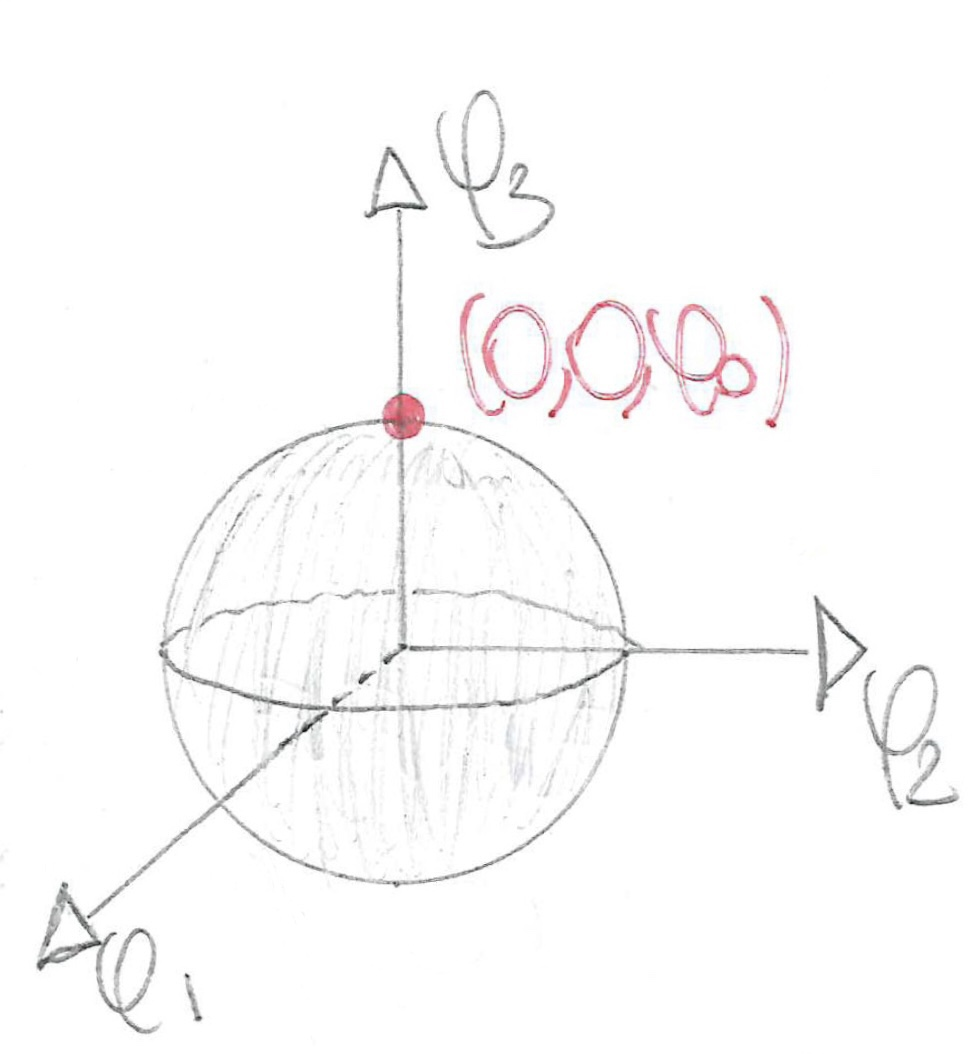
\includegraphics[]{images_ch9/2sphere_minima.jpg}}
    da cui segue che il potenziale ha un minimo in 
    \[X=  \sum_{a=1}^3\varphi^2_a = \boxed{\varphi_0^2=\frac{\mu^2}{\lambda}}\]
    L'equazione $\varphi^2_1 + \varphi^2_2 + \varphi^2_3 = \varphi^2_0$ descrive l'insieme dei possibili stati fondamentali, che geometricamente corrisponde alla 2-sfera (la superficie) di raggio $\varphi_0$, rappresentata a lato.

    Abbiamo quindi nuovamente la solita degenerazione degli stati fondamentali, tutti tra loro connessi da trasformazioni di $\textrm{SO}(3)$. Ne scegliamo uno, ad esempio il polo nord $\Vec{\varphi}_0 = (0,0,\varphi_0)$, e \textbf{questa specifica scelta rompe la simmetria originale!} 

    Tuttavia c'è un sottogruppo non banale di $\textrm{SO}(3)$ sotto il quale il vuoto risulta ancora invariante (una sorta di gruppo piccolo) e tale sottogruppo è ovviamente $\textrm{SO}(2)$, il gruppo delle rotazioni (nello spazio dei campi) attorno ad un asse specifico, in questo caso particolare $\hat{\varphi}_3$.

    Se indichiamo quindi con $T^{1,2,3}$ i generatori di $\textrm{SO}(3)$, siamo nella situazione in cui $T^{1}$ e $T^{2}$ sono rotti, mentre $T^{3}$ non lo è, in quanto genera la simmetria residua di $\textrm{SO}(2)$!
    \label{example:not_all_generators_broken}
\end{example}

Torniamo al caso generale, denominiamo con $T^a$ i generatori del gruppo $G$ (al solito $a=1,...,\dim G$) e separiamoli in $Y^a$, quelli che annichiliscono il vuoto e non sono rotti, ed in $X^a$, quelli che non lo annichiliscono, i.e. i generatori rotti. In formule:
\[
Y^a\Vec{\varphi}_0 = \Vec{0} ~,\quad X^a\Vec{\varphi}_0 \neq \Vec{0}
\]

I generatori non rotti, gli $Y^a$, formano una sottoalgebra e, di conseguenza, gli elementi generati dalla mappa esponenziale $\exp(i\alpha_aY^a)$ formano un sottogruppo di $G$, solitamente denominato “$H$”. Diciamo in generale che \textbf{la simmetria è rotta spontaneamente da $\mathbf{G}$ ad $\mathbf{H}$.}

Procediamo ora come segue:
\begin{itemize}
    \item Il potenziale è invariante sotto la simmetria globale $\textrm{SO}(3)$, quindi la sua variazione infinitesima sarà nulla e possiamo scriverla nel modo seguente:
    \begin{align*}
        0 &= \delta V(\Vec{\varphi}) =  V(\Vec{\varphi}+\delta\Vec{\varphi}) -  V(\Vec{\varphi}) \\
        &=\Ccancel[Red]{V(\Vec{\varphi})} +\frac{\partial V}{\partial\varphi_A}\delta\varphi_A -  \Ccancel[Red]{V(\Vec{\varphi})}\\
        &\overset{(\ref{eq:generalized_group_action_infinitesimal})}{=} \frac{\partial V}{\partial\varphi_A}(-i)\varepsilon_a(T^a)_{AB}\varphi_B
    \end{align*}

    Troviamo quindi:
    \[
    {\frac{\partial V}{\partial\varphi_A}\varepsilon_a(T^a)_{AB}\varphi_B = 0}
    \]
    \item Differenziamo ora rispetto a $\varphi_C$ ed eliminiamo $\varepsilon_a$, che è arbitrario, da cui segue:
    \[
    \frac{\partial^2 V}{\partial\varphi_A\partial\varphi_C}(T^a)_{AB}\varphi_B +\frac{\partial V}{\partial\varphi_A}(T^a)_{AB}\delta_{BC} = 0
    \]

    \item Possiamo ora valutare l'ultima espressione nella configurazione di vuoto $\Vec{\varphi}_0$, che per definizione annulla la derivata del potenziale! Arriviamo quindi all'equazione:
    \begin{equation}
        \boxed{\frac{\partial^2 V}{\partial\varphi_A\partial\varphi_C}(\Vec{\varphi}_0)(T^a\Vec{\varphi}_0)_A = 0}
        \label{eq:mass_matrix_=0}
    \end{equation}
    dove figura esattamente la matrice di massa, al quadrato, dei campi fisici che abbiamo discusso prima.
\end{itemize}

Ragioniamo ora sull'equazione (\ref{eq:mass_matrix_=0}) che abbiamo appena ricavato:
\begin{enumerate}
    \item[\textbf{i)}] L'equazione è banalmente soddisfatta nel caso dei generatori non rotti $Y^a$, in quanto la loro azione sulla configurazione di vuoto annulla il tutto.
    \item[\textbf{ii)}] Nel caso dei generatori rotti, tuttavia, la situazione si fa interessante (ed avrete probabilmente già capito dove stiamo andando a parare), in quanto per loro definizione $(X^a\Vec{\varphi}_0)_A \neq0$. Ciò nonostante l'equazione (\ref{eq:mass_matrix_=0}) richiede che alla fine dei conti si ottenga zero.

    \textbf{L'unica soluzione è che $X^a\Vec{\varphi}_0$ sia autovettore per la matrice di massa al quadrato, con autovalore nullo!}

    Ma allora abbiamo a che fare con un bosone di Goldstone, in quanto la sua massa è nulla. Siccome possiamo poi ripetere lo stesso argomento per ogni $X^a$, possiamo concludere che \textbf{avremo un bosone di Goldstone per ogni generatore rotto.}
\end{enumerate}
\begin{exercise}
    Mostrare che i generatori non rotti formano una sottoalgebra. \textbf{[Conti svolti Lez. 36 p. 62]}
\end{exercise}

\section[Simmetria Chirale]{$\text{SU}\text{(2)}_\text{L}\otimes \text{SU}\text{(2)}_\text{R}$ Sigma Model e Simmetria Chirale}
L'idea è a questo punto di arrivare al caso non abeliano, a tale scopo studiamo la seguente Lagrangiana:
\begin{equation}
    \boxed{\mathscr{L} = i\bar q\gamma^\mu\partial_\mu q}
    \label{eq:simplest_doublet_lagrangian}
\end{equation}
dove $q \equiv \begin{pmatrix}u\\d\end{pmatrix}$ è un doppietto di campi di Dirac (ogni campo ha 4 componenti, due sono destre e due sono sinistre).

\textbf{Qual è il gruppo di simmetria globale di questa Lagrangiana?} In primo luogo saremmo portati a dire $\textrm{SU}(2)$, sotto il quale $q$ trasforma come un doppietto e che coinvolge operatori unitari (condizione necessaria per far passare l'operatore attraverso la derivata). Questo è certamente corretto, ma c'è di più.

Prima di tutto, non abbiamo alcun motivo di restringerci al caso “speciale” del gruppo unitario, ed essendo $\dim\textrm{U}(2) = 4 > \dim\textrm{SU}(2) = 3$\footnote{Ricordiamo che $\dim\textrm{U}(N) = N^2$, mentre $\dim\textrm{SU}(N) = N^2-1$}, il gruppo $\textrm{U}(2)$ identifica un gruppo di simmetria globale più grande per la nostra Lagrangiana. Ricordiamo inoltre la valenza della relazione $\textrm{U}(2) = \textrm{U}(1)\times \textrm{SU}(2)$.

Con alcune accortezze, possiamo tuttavia scoprire informazioni ancora più interessanti.

\subsection{I Proiettori Chirali}
Introduciamo i seguenti oggetti, detti proiettori chirali:    
\begin{equation}
    \boxed{P_L \equiv \frac{1}{2}(1-\gamma^5)~,\quad P_R \equiv \frac{1}{2}(1+ \gamma^5)}
    \label{eq:chiral_projectors}
\end{equation}
Nella rappresentazione di Weyl, ricordando che $\gamma^5 = i\gamma^0\gamma^1\gamma^2\gamma^3$, abbiamo:
\begin{equation}
    \gamma^0 = \begin{pmatrix}
        0&1\\
        1&0
    \end{pmatrix}~,\quad
    \gamma^i = \begin{pmatrix}
        0&\sigma^i\\
        -\sigma^i&0
    \end{pmatrix}~\Rightarrow
    \gamma^5 = \begin{pmatrix}
        -1&0\\
        0&1
    \end{pmatrix}
    \label{eq:gammas_weyl_rep}
\end{equation}
Quindi i proiettori chirali assumono la forma esplicita:
\begin{equation}
    \boxed{P_L = \begin{pmatrix}
        1&0\\
        0&0
    \end{pmatrix} ~,\quad 
    P_R =  \begin{pmatrix}
        0&0\\
        0&1
    \end{pmatrix}}
    \label{eq:chiral_projectors_explicit}
\end{equation}

Considerando la loro applicazione su un campo di Dirac $\Psi\equiv\begin{pmatrix}\psi_L\\\psi_R\end{pmatrix}$, ovviamente troveremo:
\[
P_L\Psi = \begin{pmatrix}\psi_L\\0\end{pmatrix} \equiv \Psi_L~,\quad 
P_R\Psi = \begin{pmatrix}0\\\psi_R\end{pmatrix} \equiv \Psi_R
\]

Riprendiamo quindi la nostra trattazione in termini del doppietto $q$ e definiamo il doppietto destro ed il doppietto sinistro:
\begin{equation}
    \begin{aligned}
        &q_L\equiv P_Lq = \frac{1}{2}(1-\gamma^5)\mathbb 1_{2\times2}q = \begin{pmatrix}u_L\\d_L\end{pmatrix} \\
        &q_R\equiv P_Rq = \frac{1}{2}(1-\gamma^5)\mathbb 1_{2\times2}q = \begin{pmatrix}u_R\\d_R\end{pmatrix} 
    \end{aligned}
    \label{eq:leftright_doublet}
\end{equation}
Ricordando la proprietà elementare delle matrici $\gamma$, $\big\{\gamma^5, \gamma^\mu\big\}=0$ per ogni $\mu$, si verifica immediatamente che:
\begin{equation}
    \boxed{\gamma^\mu P_L = P_R\gamma^\mu ~,\quad \gamma^\mu P_R = P_L\gamma^\mu }
\label{eq:gamma_projectors_fliprule}
\end{equation}
così come anche $q_L+q_R = (P_L+P_R)q = q$.

\subsection{La Lagrangiana Chirale}

Raccogliendo quanto appena appreso, possiamo riscrivere la Lagrangiana iniziale, separandola nelle componenti destre e sinistre del doppietto, di cui sopravvivono solo i due termini completamente destri o sinistri, quelli misti si annullano per una combinazione delle proprietà enunciate poc'anzi.

In definitiva la Lagrangiana chirale assume la forma:
\begin{equation}
    \boxed{\mathscr{L} = i\bar q_L\gamma^\mu\partial_\mu q_L + i\bar q_R\gamma^\mu\partial_\mu q_R}
    \label{eq:chiral_lagrangian}
\end{equation}
\begin{exercise}
    Verificare che il termine $\bar q_L\gamma^\mu\partial_\mu q_R$ si annulla.
    \textbf{[Conti svolti Lez.36 p.65]}
\end{exercise}

Il fatto che nella (\ref{eq:chiral_lagrangian}) non sia presente alcun termine di massa equivale a dire che i settori destri e sinistri sono completamente disaccoppiati. Questo ci consente quindi di definire due copie di $\textrm{U}(2)$, una che lascia invariato $q_L$ e l'altra che lascia invariato $q_R$, i.e.:
\begin{center}
\begin{tabular}{l|l}
    $\mathbf{\textbf{U}(2)_L = \textbf{U}(1)_L \times \textbf{SU}(2)_L}$ & $\mathbf{\textbf{U}(2)_R = \textbf{U}(1)_R \times \textbf{SU}(2)_R}$ \\ \hline
    $q_L \rightarrow e^{-i\theta_L}e^{-i\theta_L^a{\sigma^a}/{2}}q_L$ & $q_L \rightarrow q_L$ \\
    $q_R \rightarrow q_R$ & $q_R \rightarrow e^{-i\theta_R}e^{-i\theta_R^a{\sigma^a}/{2}}q_R$ \\
\end{tabular}
\end{center}
Quindi l'effettivo gruppo di simmetria globale della Lagrangiana (\ref{eq:chiral_lagrangian}) corrisponde a $\textrm{U}(1)_L\times\textrm{U}(1)_R\times\textrm{SU}(2)_L\times\textrm{SU}(2)_R$, e da ciascuno dei gruppi che lo compongono possiamo ricavare le rispettive correnti di Noether. Non è difficile convincersi che questo siano:
\[\boxed{\begin{aligned}
    &\textrm{U}(1)_L  \rightarrow j^\mu_L = \bar q_L \gamma^\mu q_L    \\
    &\textrm{U}(1)_R  \rightarrow j^\mu_R = \bar q_R \gamma^\mu q_R    \\
    &\textrm{SU}(2)_L \rightarrow j^{a,\mu}_L = \bar q_L \gamma^\mu \frac{\sigma^a}{2}q_L    \\
    &\textrm{SU}(2)_R \rightarrow j^{a,\mu}_R = \bar q_R \gamma^\mu \frac{\sigma^a}{2}q_R   
\end{aligned}}\]

\subsection{Simmetria Vettoriale ed Assiale}
Invece di separare la Lagrangiana in componenti destre e sinistre, continuiamo a lavorare con $\mathscr{L} = i\bar q\gamma^\mu\partial_\mu q$ e cerchiamo di capire dove sia nascosto il gruppo di simmetria che abbiamo appena scoperto.

Non c'è dubbio sul fatto che questa Lagrangiana possieda una simmetria sotto il gruppo $\textrm{U}(2) \equiv \textrm{U}(2)_V$ dove $V$ sta per \textbf{vettoriale} e dove con trasformazione “vettoriale” intendiamo una trasformazione del tipo
\(q \rightarrow e^{-i\theta_V}e^{-i\theta_V^a{\sigma^a}/{2}}q\).

Ovviamente a tale gruppo di simmetria corrispondono delle correnti di Noether, la cui struttura è la stessa di quelle che abbiamo già visto poco fa, a meno del pedice che in questo caso sarà $V$.

\begin{exercise}
    Mostrare che le cariche $Q_V = \int_{}d^3\Vec{x}\,j^{a,0}_V(x)$ chiudono l'algebra di $\textrm{SU}(2)$. \textbf{[Conti svolti Lez. 36 p. 67÷68]}
    \label{ex:QV_SU2_algebra}
\end{exercise}

Consideriamo ora una trasformazione leggermente differente, aggiungendo $\gamma^5$ negli esponenziali, i.e.: 

\[\boxed{\begin{aligned}
    &q \rightarrow e^{-i\theta_A\gamma^5}e^{-i\theta_A^a\frac{\sigma^a}{2}\gamma^5}q\\
    &\bar{q} \rightarrow \bar{q}e^{-i\theta_A\gamma^5}e^{-i\theta_A^a\frac{\sigma^a}{2}\gamma^5}
\end{aligned}}\]
dove la legge di trasformazione per l'aggiunto di Dirac segue dalla prima per mezzo dell'anti-commutazione tra $\gamma^5$ e tutte le altre $\gamma$.

Si verifica che il gruppo a cui fa capo una tale trasformazione, $\textrm{U}(2)_A$, è un gruppo di simmetria per la nostra Lagrangiana. Questa simmetria è detta simmetria “\textbf{assiale}”, da cui i pedici $A$, ed anche in questo caso avremo una corrente da $\textrm{U}(1)_A$ e tre correnti da $\textrm{SU}(2)_A$. 

Riassumendo:
\begin{center}
\begin{tabular}{l|l}
    $\mathbf{\textbf{U}(2)_V = \textbf{U}(1)_V \times \textbf{SU}(2)_V}$ & $\mathbf{\textbf{U}(2)_A = \textbf{U}(1)_A \times \textbf{SU}(2)_A}$ \\ \hline
    $q \rightarrow e^{-i\theta_V}e^{-i\theta_V^a{\sigma^a}/{2}}q$ &  $q \rightarrow e^{-i\theta_A\gamma^5}e^{-i\theta_A^a\frac{\sigma^a}{2}\gamma^5}q$ \\
    $\textrm{U}(1)_V  \Rightarrow j^\mu_V = \bar q \gamma^\mu q$    & $\textrm{U}(1)_A  \Rightarrow j^{\mu}_A = \bar q \gamma^\mu\gamma^5 q$   \\
    $\textrm{SU}(2)_V  \Rightarrow j^\mu_V = \bar q \gamma^\mu q$    & $\textrm{SU}(2)_A  \Rightarrow j^{a,\mu}_A = \bar q \frac{\sigma^a}{2}\gamma^\mu\gamma^5 q$ 
\end{tabular}
\end{center}

\subsubsection{$\star$\underline{Simmetria U(1) Vettoriale ed Assiale}}
A questo punto è utile riscrivere le trasformazioni di $\textrm{U}(1)_V$ ed $\textrm{U}(1)_A$ in termini della loro azione sulle componenti destre e sinistre:
\begin{itemize}
    \item \textbf{Per la trasformazione vettoriale} abbiamo $q\rightarrow e^{-i\theta_V}q$.

    Applicando i proiettori chirali otteniamo banalmente l'azione di $\textrm{U}(1)_V$ sulle componenti destre e sinistre, che risultano in defnitiva ruotate dello stesso angolo, i.e.:
    \[
    \boxed{
    \textrm{U}(1)_V ~:~
    \begin{aligned}
        &q_L\rightarrow e^{-i\theta_V}q_L\\
        &q_R\rightarrow e^{-i\theta_V}q_R
    \end{aligned}}
    \]
    
    \item \textbf{Per la trasformazione assiale}, d'altro canto, dobbiamo porre più attenzione. La trasformazione di base è $q\rightarrow e^{-i\theta_A\gamma^5}q$ e la presenza di $\gamma^5$ va tenuta in considerazione quando andiamo ad applicare i proiettori chirali.

    Alla fine dei conti la sostanza è che per invertire l'ordine tra il proiettore sinistro e l'operatore di $\textrm{U}(1)_A$ bisogna eliminare la $\gamma^5$ e cambiare di segno all'esponente, mentre per fare la stessa cosa con il proiettore destro il segno non va cambiato. In formule:
    \[
    \boxed{
    \textrm{U}(1)_A ~:~
    \begin{aligned}
        &q_L\rightarrow e^{i\theta_A}q_L\\
        &q_R\rightarrow e^{-i\theta_A}q_R
    \end{aligned}}
    \]
    Ergo, sotto l'azione di $\textrm{U}(1)_A$, fermioni destri e sinistri vengono ruotati di fasi opposte.
\end{itemize}
Considerando allora l'azione combinata $\textrm{U}(1)_V\times \textrm{U}(1)_A$, nel caso in cui $\theta_A=\theta_V \equiv \theta_R/2$, siamo sostanzialmente di fronte all'azione del gruppo $\textrm{U}(1)_R$, infatti:
\[
\boxed{
\begin{aligned}
    \textrm{U}(1)_V&\times \textrm{U}(1)_A \\
    \theta_A=&\theta_V \equiv {\theta_R}/2
\end{aligned}~:~
\begin{aligned}
    &q_L\rightarrow e^{-i\theta_R/2}e^{i\theta_R/2}q_L = q_L\\
    &q_R\rightarrow e^{-i\theta_R/2}e^{-i\theta_R/2}q_R = e^{-i\theta_R}q_R
\end{aligned}}\equiv \textrm{U}(1)_R
\]

Considerando invece l'azione combinata $\textrm{U}(1)_V\times \textrm{U}(1)_A$, nel caso in cui $\theta_A=-\theta_V \equiv -\theta_L/2$, siamo di fronte all'azione del gruppo $\textrm{U}(1)_R$:
\[
\boxed{
\begin{aligned}
    \textrm{U}(1)_V&\times \textrm{U}(1)_A \\
   \theta_A=-&\theta_V \equiv -\theta_L/2
\end{aligned}~:~
\begin{aligned}
    &q_L\rightarrow e^{-i\theta_L/2}e^{-i\theta_L/2}q_L = e^{-i\theta_L}q_L\\
    &q_R\rightarrow e^{-i\theta_L/2}e^{i\theta_L/2}q_R = q_R
\end{aligned}}\equiv \textrm{U}(1)_L
\]
Questo significa che $\textrm{U}(1)_L\times \textrm{U}(1)_R\cong \textrm{U}(1)_V\times \textrm{U}(1)_A$ e la differenza sta nella differente scelta dei generatori.

Dal punto di vista delle cariche, abbiamo:
\begin{align*}
    &Q_V \equiv \int_{}d^3\Vec{x}\,\bar q\gamma^0 q &Q_A \equiv \int_{}d^3\Vec{x}\,\bar q\gamma^0\gamma^5 q\\
    &Q_L \equiv \int_{}d^3\Vec{x}\,\bar q_L\gamma^0 q_L &Q_R \equiv \int_{}d^3\Vec{x}\,\bar q_R\gamma^0 q_R
\end{align*}
e si verifica quasi immediatamente, utilizzando le regole dei proiettori ed esplicitando la presenza di $q$ nelle cariche $L$ ed $R$, che:
\begin{align*}
    &Q_L+Q_R = Q_V    &Q_R-Q_L = Q_A
\end{align*}

Il cambio di base è quindi:
\begin{equation}
   \boxed{
    \begin{cases}
        Q_V = Q_L + Q_R\\
        Q_A = Q_R - Q_L
    \end{cases}\rightarrow
    \begin{cases}
        Q_R = (Q_A + Q_V)/2\\
        Q_L = (Q_V - Q_A)/2
    \end{cases}} 
    \label{eq:basis_change_VA_LR}
\end{equation}

\subsubsection{$\star$\underline{Simmetria SU(2) Vettoriale ed Assiale}}

Per quanto riguarda le cariche derivanti da $\textrm{SU}(2)$, si può verificare che queste, nel caso della simmetria assiale e vettoriale, rispettano le seguenti algebre:
\begin{equation}
    \begin{aligned}
        &\big[Q_A^a,Q_A^b\big] = i\varepsilon^{abc}Q_V^c \\
        &\big[Q_V^a,Q_V^b\big] = i\varepsilon^{abc}Q_V^c \\
        &\big[Q_V^a,Q_A^b\big] = i\varepsilon^{abc}Q_A^c
    \end{aligned}
    \label{eq:vectoraxial_charges_algebra}
\end{equation}
\begin{exercise}
    Verificare la prima e l'ultima delle (\ref{eq:vectoraxial_charges_algebra}), la seconda è il risultato dell'esercizio \ref{ex:QV_SU2_algebra}. \textbf{[Conti svolti Lez.36 p.72÷73]}
\end{exercise}

Adottando quindi il cambiamento di base (\ref{eq:basis_change_VA_LR}) scopriamo che l'algebra 6-dimensionale generata da $Q_V^a$ e $Q_A^a$ è equivalente all'algebra 6-dimensionale di $\textrm{SU}(2)_L\times \textrm{SU}(2)_R$, i.e.:
\begin{equation}
    \begin{aligned}
        &\big[Q_L^a,Q_L^b\big] = i\varepsilon^{abc}Q_L^c \\
        &\big[Q_R^a,Q_R^b\big] = i\varepsilon^{abc}Q_R^c \\
        &\big[Q_L^a,Q_R^b\big] = 0
    \end{aligned}
    \label{eq:leftright_charges_algebra}
\end{equation}
\begin{exercise}
    Scrivere l'azione delle trasformazioni vettoriali ed assiali, nel caso di $\textrm{SU}(2)$, in termini dei campi destri e sinistri $q_R$ e $q_L$. \textbf{[Conti svolti Lez.36 p.75÷76]}

    \textbf{Soluzione. } La logica è analoga a quella usata per riscrivere l'azione combinata vettoriale-assiale, solo che in questo caso consideriamo le singole azioni in funzione dei parametri $\theta_V^a$ e $\theta_A^a$. 

    Alla fine dei conti i risultati sono i seguenti:
    \begin{center}
    \begin{tabular}{l|l}
        ${\textbf{SU}\mathbf{(2)_V}}$ & ${\textbf{SU}\mathbf{(2)_A}} $ \\ \hline
         $V(\Vec{\theta}_V)\equiv\exp(-i\theta_V^a\frac{\sigma^a}{2})$ & $A(\Vec{\theta}_A) \equiv \exp(-i\theta_A^a\frac{\sigma^a}{2})$\\
        $q_L \rightarrow V(\Vec{\theta}_V)q_L$ &  $q_L \rightarrow A(\Vec{\theta}_A)^\dagger q_L$ \\
        $q_R \rightarrow V(\Vec{\theta}_V)q_R$ &  $q_R \rightarrow A(\Vec{\theta}_A)q_R$
    \end{tabular}
    \end{center}
    Da queste trasformazioni ci accorgiamo che un termine di massa del tipo $m\bar q q$ sarebbe compatibile con le trasformazioni vettoriali, ma non con quelle assiali. È quindi proprio la simmetria assiale ad impedire la presenza del termine di massa!
    \label{ex:axial_vectorial_SU2transf_chiral}
\end{exercise}

\subsection{$\text{SU}\text{(2)}_\text{L}\otimes \text{SU}\text{(2)}_\text{R}$ Sigma Model}

Partendo dalla semplice Lagrangiana studiata fino ad ora, la (\ref{eq:simplest_doublet_lagrangian}), “allarghiamo” la teoria, inserendo termini composti da campi scalari $\phi$ e $\varphi$, così come anche un potenziale ed un termine di interazione tra scalari e fermioni. Vogliamo sostanzialmente studiare la seguente teoria:
\begin{equation}
    \boxed{\begin{aligned}
        \mathscr{L} = &\frac{1}{2}\textcolor{Red}{\bigg[(\partial_\mu\varphi)(\partial^\mu\varphi) + \sum_{a=1}^3(\partial_\mu\phi_a)(\partial^\mu\phi_a)\bigg]} + i\bar q\gamma^\mu\partial_\mu q  +\\
        &+ \mathsf{g}\textcolor{Green}{\bar q\big(\varphi +i\gamma^5\Vec{\sigma}\cdot\vec{\phi}\big) q} +\frac{\mu^2}{2}\textcolor{blue}{\bigg(\varphi^2 + \sum_{a=1}^3\phi_a^2\bigg)} -\frac{\lambda}{4}\textcolor{blue}{\bigg(\varphi^2 + \sum_{a=1}^3\phi_a^2\bigg)^2}
    \end{aligned}}
    \label{eq:enlarged_lagrangian}
\end{equation}

Risulta conveniente riscrivere i termini scalari utilizzando la seguente matrice $2\times2$:
\begin{equation}
    \boxed{\Sigma \equiv \varphi\mathbb1_{2\times2} + i\Vec{\sigma}\cdot\vec{\phi}}
    \label{eq:scalar_terms_redefined}
\end{equation}

L'utilità di questa scrittura si manifesta nei modi seguenti:
\begin{itemize}
    \item Innanzitutto, ricordando che le matrici di Pauli $\Vec{\sigma}$ sono Hermitiane e ricordandone le relazioni di (anti-)commutazione, riassunte in $\sigma^a\sigma^b = \delta^{ab}\mathbb1 + i\varepsilon^{abc}\sigma^c$, si trova:
    \[
    \Sigma\Sigma^\dagger = \varphi^2\mathbb1 + \phi_a\phi_b\big(\delta^{ab}\mathbb1 + i\varepsilon^{abc}\sigma^c\big)
    \]
    Ma il termine in $\varepsilon^{abc}$ (antisimmetrico sotto $a \leftrightarrow b$) è moltiplicato a $\phi_a\phi_b$ (simmetrico sotto $a \leftrightarrow b$), quindi non contribuisce.
    In definitiva abbiamo:
    \[
    \Sigma\Sigma^\dagger = \big(\varphi^2 + \Vec{\phi}\cdot\Vec{\phi}\big)\mathbb1
    \]

    \item Alla luce del risultato del punto precedente, di cui ora prendiamo la traccia, troviamo la prima relazione interessante:
    \begin{equation}
        \boxed{\textcolor{blue}{\Tr[\Sigma\Sigma^\dagger]} = 2\bigg(\varphi^2 + \sum_{a=1}^3\phi_a\phi_a\bigg)}
        \label{eq:SigmaSigma_trace}
    \end{equation}

    \item D'altro canto, considerando la derivata di $\Sigma$:
    \[
    \partial_\mu \Sigma= \partial_\mu\varphi\mathbb1_{2\times2} + i\Vec{\sigma}\cdot\partial_\mu\vec{\phi}
    \]
    Non è difficile concludere che:
    \[
    \big(\partial_\mu \Sigma\big)\big(\partial^\mu \Sigma^\dagger\big) = \big[\big(\partial_\mu \varphi\big)\big(\partial^\mu \varphi\big) + \big(\partial_\mu \vec{\phi}\big)\big(\partial^\mu \vec{\phi}\big)\big]\mathbb1_{2\times2}
    \]
    e di conseguenza:
    \begin{equation}
        \boxed{\textcolor{Red}{\Tr[\big(\partial_\mu \Sigma\big)\big(\partial^\mu \Sigma^\dagger\big)]} = 2\bigg[\big(\partial_\mu \varphi\big)\big(\partial^\mu \varphi\big) + \sum_{a=1}^3\big(\partial_\mu \phi_a\big)\big(\partial^\mu \phi_a\big)\bigg]}
        \label{eq:derSigmaderSigma_trace}
    \end{equation}

    \item Se ora consideriamo $\bar q_L\Sigma q_R$ e $\bar q_R\Sigma^\dagger q_L$, riscrivendo $q_{L,R}$ ed aggiunti in termini di $P_{L,R}q$, ricordando il fatto che $\bar q_L = \bar q P_R$ (viceversa per $\bar q_R$) e notando il fatto che i proiettori chirali sono idempotenti (i.e. $P_{L,R}^2=P_{L,R}$), si trova:
    \begin{align*}
        &\bar q_L\Sigma q_R = \bar q \big(\varphi\mathbb1_{2\times2} + i\Vec{\sigma}\cdot\vec{\phi}\big) P_R q\\
        &\bar q_R\Sigma^\dagger q_L = \bar q \big(\varphi\mathbb1_{2\times2} - i\Vec{\sigma}\cdot\vec{\phi}\big) P_L q
    \end{align*}

    Di conseguenza, sfruttando il fatto che $P_R+P_L=1$ e  $P_R-P_L=\gamma^5$, è chiaro che:

    \begin{equation}
        \boxed{
        \textcolor{Green}{\bar q_L\Sigma q_R + \bar q_R\Sigma^\dagger q_L} = \bar q \big(\varphi\mathbb1_{2\times2} + i\gamma^5\Vec{\sigma}\cdot\vec{\phi}\big) q
        }
        \label{eq:sigma_interaction_leftright}
    \end{equation}
\end{itemize}

Possiamo quindi riscrivere la Lagrangiana (\ref{eq:enlarged_lagrangian}):
\begin{equation}
    \boxed{\begin{aligned}
        \mathscr{L} = &\frac{1}{4}\Tr[\big(\partial_\mu \Sigma\big)\big(\partial^\mu \Sigma^\dagger\big)] + i\bar q\gamma^\mu\partial_\mu q  +\\
        &+ \mathsf{g}\big(\bar q_L\Sigma q_R + \bar q_R\Sigma^\dagger q_L\big) +\frac{\mu^2}{4}\Tr[\Sigma\Sigma^\dagger] -\frac{\lambda}{16}{\Big(\Tr[\Sigma\Sigma^\dagger]\Big)^2}
    \end{aligned}}
    \label{eq:enlarged_lagrangian_sigma}
\end{equation}
Ora le simmetrie sono più evidenti:
\begin{enumerate}
    \item[\textbf{i)}] \textbf{La Lagrangiana è invariante sotto le trasformazioni di SU$\mathbf{(2)_V}$ estese al campo scalare}, i.e.:
    \begin{equation}
        \boxed{\begin{aligned}
            &V(\Vec{\theta}_V) \equiv \exp(-i\Vec{\theta}_V\cdot\frac{\Vec{\sigma}}{2})\\
             q\rightarrow V(\Vec{\theta}_V) q&~,\quad \bar q\rightarrow \bar q V(\Vec{\theta}_V)^\dagger~,\quad \Sigma\rightarrow \Sigma'= V\Sigma V^\dagger
        \end{aligned}}
        \label{eq:SU2_V_enlargedlagrangian_symmetry}
    \end{equation}
    \begin{proof}
        L'unica invarianza non del tutto banale è quella del termine di interazione, in cui va tenuto conto del fatto che:
        \[
        q_L\rightarrow V(\Vec{\theta}_V) q_L ~,\quad q_R\rightarrow V(\Vec{\theta}_V) q_R
        \]
        Dato ciò, il resto dei conti è banale.
    \end{proof}
    \begin{nota}
        Considerando la trasformazione di $\Sigma$ espandendo quest'ultima secondo la (\ref{eq:scalar_terms_redefined}), possiamo evidenziare alcuni fatti interessanti.

        Il primo risultato viene dal termine in $\varphi$:
        \begin{equation}
            \boxed{\varphi \rightarrow V\varphi V^\dagger = \varphi}
            \label{eq:varphi_is_SU2_V_singlet}
        \end{equation}
        i.e. $\varphi$ è un singoletto sotto SU$(2)_V$!

        Per quanto riguarda invece il secondo termine, proviamo ad isolare la proprietà di trasformazione di $\phi_a$ partendo da:
        \[
        \Vec{\phi}\cdot\Vec{\sigma} \rightarrow V\Vec{\phi}\cdot\Vec{\sigma} V^\dagger
        \]
        Sottintendendo le somme sugli indici ripetuti, al LHS abbiamo semplicemente $\phi_a\sigma^a$, mentre sul RHS, che scriviamo
        \[
        e^{-i\Vec{\theta}_V\cdot\Vec{\sigma}/{2}}\phi_a\sigma^a e^{i\Vec{\theta}_V\cdot\Vec{\sigma}/{2}}
        \]
        possiamo lavorare applicando la formula di \href{https://it.wikipedia.org/wiki/Formula_di_Baker-Campbell-Hausdorff}{Baker-Campbell-Hausdorff}, i.e.:
        \begin{equation}
            \begin{aligned}
                e^{iA}Be^{-iA} =& B +i\big[A,B\big] + \frac{i^2}{2!}\big[A,\big[A,B\big]\big] + \cdots +\\
                &+\frac{i^n}{n!}\big[A,\big[A, \cdots \big[A,B\big]\big]\big]+ \cdots
            \end{aligned}
            \label{eq:BCH_formula}
        \end{equation}
        identificando nel nostro caso specifico $A\equiv -\Vec{\theta}_V\cdot\Vec{\sigma}/{2}$ e $B\equiv \sigma^a$.

        Il commutatore ed il doppio vanno calcolati a mano, definendo $\big(T_\text{adj}^a\big)_bc\equiv -i\varepsilon^{abc}$, e i risultati a cui si arriva sono i seguenti:
        \[
        \begin{cases}
            \big[-\Vec{\theta}_V\cdot{\Vec{\sigma}}/{2},\sigma^a\big] = \theta_V^b\big(T_\text{adj}^b\big)_{ac}\sigma^c \\
            \big[-\Vec{\theta}_V\cdot{\Vec{\sigma}}/{2},\big[-\Vec{\theta}_V\cdot{\Vec{\sigma}}/{2},\sigma^a\big]\big] = \big(\Vec{\theta}_V\cdot\Vec{T}_\text{adj}\big)^2_{ac}\sigma^c
        \end{cases}
        \]

        Applicando quindi la BCH al caso di nostro interesse, otteniamo quanto segue:
        \begin{align*}
            \phi_a e^{-i\Vec{\theta}_V\cdot\Vec{\sigma}/{2}}\sigma^a e^{i\Vec{\theta}_V\cdot\Vec{\sigma}/{2}} =\phi_a\big\{& \sigma^a + i \theta_V^b\big(T_\text{adj}^b\big)_{ac}\sigma^c +\\
            & + i\big(\Vec{\theta}_V \cdot \Vec{T}_\text{adj} \big)^2_{ac} \sigma^c + \cdots \big\}
        \end{align*}
        Notiamo quindi che gli elementi tra parentesi graffa ricostruiscono un esponenziale! Questo ci permette di riscrivere la legge di trasformazione da cui siamo partiti:
        \[
        \phi_c\sigma^c \rightarrow  \phi_a\big[\exp\big(i\Vec{\theta}_V \Vec{T}_\text{adj})\big]_{ac}\sigma^c
        \]
        Per poi usare l'anti-simmetria di $\Vec{T}_\text{adj}$ sotto $a\leftrightarrow c$ arrivando in definitiva alla conclusione che $\Vec\phi$ trasforma sotto la rappresentazione aggiunta di SU$(2)_V$, i.e.:
        \begin{equation}
            \boxed{\phi_c \rightarrow \big[\exp\big(-i\Vec{\theta}_V \Vec{T}_\text{adj})\big]_{ca} \phi_a}
            \label{eq:phi_SU2_V_adjoint_transform}
        \end{equation}
        \label{note:singlet_and_adjoint}
    \end{nota}
    
    Se ora prendiamo la forma infinitesima della (\ref{eq:phi_SU2_V_adjoint_transform}), troviamo:
    \[
    \phi_c \rightarrow\big[\delta_{ca} - i \theta_V^A(T_\text{adj}^A)_{ca}\big]\phi_a = \phi_c -\theta_V^A\varepsilon^{Aca}\phi_a
    \]
    Quindi giocando opportunamente con gli indici troviamo la forma della variazione infinitesima di $\Vec{\phi}$:
    \begin{equation}
        \boxed{\begin{aligned}
            &\delta\phi_c = -\theta_V^a\varepsilon^{acb}\phi_b = \varepsilon^{cab}\theta_V^a\phi_b \\
            &\Rightarrow ~\delta\Vec{\phi} = \Vec{\theta}\times \Vec{\phi} 
        \end{aligned}}
        \label{eq:infinitesimal_phi_variation}
    \end{equation}
    Possiamo quindi calcolare la corrente conservata associata ad SU$(2)_V$, che in linea del tutto generale si scrive:
    \[
    V^{a,\mu} = \frac{\partial\mathscr{L}}{\partial(\partial_\mu q)}\frac{\delta q}{\delta\theta^A_V} + \frac{\partial\mathscr{L}}{\partial(\partial_\mu \varphi)}\frac{\delta \varphi}{\delta\theta^A_V} +\frac{\partial\mathscr{L}}{\partial(\partial_\mu\Vec{\phi})}\frac{\delta \Vec\phi}{\delta\theta^A_V}
    \]
    Chiaramente $\delta q = -i\theta_V^A\frac{\sigma^A}{2}q$ ed altrettanto chiaramente il secondo termine è nullo in quanto $\varphi$ è un singoletto sotto SU$(2)_V$. Di conseguenza, la corrente di Noether si scrive:
    \begin{equation}
        \begin{aligned}
            &V^{a,\mu} = \bar q \gamma^\mu\frac{\sigma^A}{2} q + (\partial^\mu\phi_c)\varepsilon^{cAb}\phi_b = \bar q \gamma^\mu\frac{\sigma^A}{2} q - (\partial^\mu\phi_c)\varepsilon^{Acb}\phi_b\\
            &\Rightarrow ~\boxed{\Vec{V}^{\mu} \equiv \bar q \gamma^\mu\frac{\sigma^A}{2} q - (\partial^\mu\Vec{\phi})\times \Vec{\phi}}
        \end{aligned}
        \label{eq:SU2_V_noethercurrent}
    \end{equation}

    A cui associamo la carica conservata \(\Vec{Q}_V \equiv \int_{}d^3\Vec{x}\, V^0(\Vec{x},t)\) .

    
    \item[\textbf{ii)}] \textbf{La Lagrangiana è invariante sotto le trasformazioni di SU$\mathbf{(2)_A}$ estese al campo scalare}, i.e.:
    \begin{equation}
        \boxed{\begin{aligned}
            &A(\Vec{\theta}_A) \equiv \exp(-i\Vec{\theta}_A\cdot\frac{\Vec{\sigma}}{2})\\
             q\rightarrow \exp(-i\Vec{\theta}_A\cdot\frac{\Vec{\sigma}}{2}\gamma^5) q&~,\quad \Sigma\rightarrow \Sigma'= A^\dagger\Sigma A^\dagger
        \end{aligned}}
        \label{eq:SU2_A_enlargedlagrangian_symmetry}
    \end{equation}

    \begin{proof}
        Anche qui l'invarianza è evidente, l'unica accortezza da tenere è nel caso del termine di interazione in cui vanno applicate le regole di trasformazione ricavate nell'esercizio \ref{ex:axial_vectorial_SU2transf_chiral}.
    \end{proof}

    Anche in questo caso vorremmo esplicitare quali siano le correnti di Noether e per farlo dobbiamo trovare le variazioni infinitesime di $\varphi$ e $\Vec{\phi}$, in quanto ancora una volta quella di $q$ la conosciamo già. 

    Per trovare tali variazioni lavoriamo nuovamente sulla trasformazione di $\Sigma$ espandendo gli $A^\dagger$ nel caso infinitesimo e svolgendo i prodotti, eventualmente tenendo conto delle regole di anticommutazione delle matrici di Pauli. I calcoli sono lasciati per esercizio \textbf{[Conti svolti Lez. 37 p.83÷84]} ma il risultato a cui si arriva è il seguente:
    \[
    \Sigma = \varphi +i\Vec\sigma\cdot\Vec\phi \xrightarrow{\text{SU}(2)_A} \varphi - \Vec\phi\cdot\Vec{\theta}_A +i(\Vec{\phi} +\varphi\Vec{\theta}_A)\cdot\Vec\sigma
    \]

    A questo punto abbiamo tutte le variazioni che ci servono:
    \begin{equation}
        \boxed{\delta q = -i\theta_A^a\frac{\sigma^a}{2}\gamma^5 q~,\quad
        \delta \varphi = - \phi_a\theta_A^a~,\quad
        \delta\phi_a = \varphi\theta^a_A}
        \label{eq:SU2_A_infinit_fields_variation}
    \end{equation}
    Possiamo dunque scrivere la corrente di Noether:
    \begin{align*}
        A^{a,\mu} &=\frac{\partial\mathscr{L}}{\partial(\partial_\mu q)}\frac{\delta q}{\delta\theta^a_A} + \frac{\partial\mathscr{L}}{\partial(\partial_\mu \varphi)}\frac{\delta \varphi}{\delta\theta^a_A} +\frac{\partial\mathscr{L}}{\partial(\partial_\mu\Vec{\phi})}\frac{\delta \Vec\phi}{\delta\theta^a_A}\\
        &= \bar q\gamma^\mu\frac{\sigma^A}{2}\gamma^5 q + (\partial^\mu\varphi)(-\phi_a) + (\partial^\mu\phi_a)\varphi
    \end{align*}

    Quindi in definitiva:
    \begin{equation}
        \boxed{\Vec{A}^{\mu} = \bar q\gamma^\mu\frac{\Vec{\sigma}}{2}\gamma^5 q - \big[\Vec{\phi}(\partial^\mu\varphi) - \varphi(\partial^\mu\Vec{\phi})\big]}
        \label{eq:SU2_A_noethercurrent}
    \end{equation}
    A cui associamo la carica \(\Vec{Q}_A \equiv \int_{}d^3\Vec{x}\, A^0(\Vec{x},t)\) .
\end{enumerate}

Si dimostra che le cariche conservate associate ad SU$(2)_{V,A}$ soddisfano le seguenti algebre:
\begin{equation}
    \boxed{\begin{aligned}
        \big[{Q}^a_V,{Q}^b_V\big] = i\varepsilon^{abc}Q^c_V~,\quad
        \big[{Q}^a_A,{Q}^b_A\big] = i\varepsilon^{abc}Q^c_V~,\quad
        \big[{Q}^a_V,{Q}^b_A\big] = i\varepsilon^{abc}Q^c_A
    \end{aligned}}
    \label{eq:vector_axial_SU2charges_algebra}
\end{equation}

Possiamo allora definire nuovamente 
\[
\Vec{Q}_R = (\Vec{Q}_A + \Vec{Q}_V)/2~,\quad \Vec{Q}_L = (\Vec{Q}_V - \Vec{Q}_A)/2
\]

E verificare che $\Vec{Q}_L$ e $\Vec{Q}_R$ chiudono entrambe l'algebra di SU$(2)_L\times$SU$(2)_R$, i.e.:
\begin{equation}
    \boxed{\begin{aligned}
        \big[{Q}^a_L,{Q}^b_L\big] = i\varepsilon^{abc}Q^c_L~,\quad
        \big[{Q}^a_R,{Q}^b_R\big] = i\varepsilon^{abc}Q^c_R~,\quad
        \big[{Q}^a_L,{Q}^b_R\big] = 0
    \end{aligned}}
    \label{eq:leftright_SU2charges_algebra}
\end{equation}

Notiamo inoltre come SU$(2)_V$ sia un sottogruppo di SU$(2)_L\times$SU$(2)_R$, noto come \textbf{sottogruppo diagonale}.

\begin{nota}
    Sulla scia di quanto già visto nel caso di U$(1)_{V,A}$, possiamo studiare l'azione combinata assiale vettoriale su $q_{L,R}$ nel caso di SU$(2)$.

    I ragionamenti sono pressoché gli stessi, e quello che si trova alla fine dei conti è che:
    \begin{itemize}
    \item Se si considera $\Vec\theta_V=\Vec\theta_A \equiv \Vec\theta_R/2$, l'azione combinata assiale-vettoriale su $q_{L,R}$ corrisponde all'azione di SU$(2)_R$. 

    \item D'altro canto, considerando $\Vec\theta_V=-\Vec\theta_A \equiv \Vec\theta_L/2$, l'azione combinata assiale-vettoriale su $q_{L,R}$ corrisponde all'azione di SU$(2)_L$.
    \end{itemize}

    Ci si potrebbe chiedere a questo punto cosa accada a $\Sigma$, la cui legge di trasformazione sotto la combinazione assiale-vettoriale diventa:
    \[
    \Sigma \rightarrow V(A^\dagger\Sigma A^\dagger)V^\dagger
    \]
    ci accorgiamo senza troppa difficoltà che:
    \begin{itemize}
        \item Se $\Vec\theta_V=\Vec\theta_A\equiv \Vec\theta_R/2$
        \begin{align*}
            &\Sigma \rightarrow \Sigma\big[\exp\big(-i\Vec\theta_R\cdot\Vec{\sigma}/2)\big]^\dagger \equiv \Sigma R(\Vec\theta_R)^\dagger \\
            &R(\Vec\theta_R) \in \text{SU}(2)_R
        \end{align*}
        \item Se $\Vec\theta_V=-\Vec\theta_A\equiv \Vec\theta_L/2$
        \begin{align*}
            &\Sigma \rightarrow \exp\big(-i\Vec\theta_L\cdot\Vec{\sigma}/2\big) \Sigma\equiv L(\Vec\theta_L)\Sigma \\
            &L(\Vec\theta_L) \in \text{SU}(2)_L
        \end{align*}
    \end{itemize}
    Questo significa che, sotto l'azione di SU$(2)_L\times$SU$(2)_R$, $\Sigma$ trasforma secondo:
    
    \[\boxed{\Sigma \rightarrow L\Sigma R^\dagger}\]
    con
    \begin{align*}
        L(\Vec\theta_L) = \exp\big(-i\Vec\theta_L\cdot\Vec{\sigma}/2\big) ~, \quad R(\Vec\theta_R) = \exp\big(-i\Vec\theta_R\cdot\Vec{\sigma}/2\big)
    \end{align*}
    Questa è detta rappresentazione bi-fondamentale di  SU$(2)_L\times$SU$(2)_R$.
    \label{note:bifundamental_repres}
\end{nota}

\subsection{Rottura spontanea della simmetria chirale}

Consideriamo a questo punto il potenziale che abbiamo introdotto nella Lagrangiana chirale generalizzata (\ref{eq:enlarged_lagrangian}), i.e.:
\begin{equation}
    \begin{aligned}
        V &= - \frac{\mu^2}{2}\bigg(\varphi^2 + \sum_{a=1}^3\phi_a^2\bigg) + \frac{\lambda}{4}\bigg(\varphi^2 + \sum_{a=1}^3\phi_a^2\bigg)^2\\
        &=\frac{\mu^2}{4}\Tr[\Sigma\Sigma^\dagger] -\frac{\lambda}{16}\Big(\Tr[\Sigma\Sigma^\dagger]\Big)^2
    \end{aligned}
    \label{eq:chiral_potential}
\end{equation}
Notando la dipendenza del potenziale dal solo $|\varphi|$ possiamo sfruttare la solita procedura per ricavare che questo possiede un set di minimi degeneri in:
\[
\varphi^2 + \sum_{a=1}^3\phi_a^2 = \frac{\mu^2}{\lambda} \equiv \varphi_0^2
\]
tutti legati da trasformazioni di SO$(4)$.

Possiamo dunque fare una scelta e fissare il vuoto in modo tale che:
\[
\langle0|\varphi|0\rangle = \varphi_0~,\quad\langle0|\Vec\phi|0\rangle=\Vec{0}
\]
che in termini di un vettore 4-dimensionale $\Vec\Phi \equiv \begin{pmatrix}\varphi \\ \Vec{\phi}\end{pmatrix}$ si scrive:
\begin{equation}
    \langle0|\Vec\Phi|0\rangle = \begin{pmatrix}\varphi_0 \\ \Vec{0}\end{pmatrix}
    \label{eq:vacuum_choice_chiral}
\end{equation}
Questo stato di vuoto è chiaramente invariante sotto le trasformazioni di SO$(3)$, quindi \textbf{questa scelta genera una rottura spontanea di simmetria SO$\mathbf{(4)}\rightarrow$SO$\mathbf{(3)}$}.

Ora qualcuno qui potrebbe chiedersi cosa c'entrino SO$(4)$ ed SO$(3)$, visto che abbiamo dedicato le precedenti pagine alla discussione del modello SU$(2)_L\times$SU$(2)_R$. 

Il punto sta nel fatto che sussiste un isomorfismo tra i seguenti gruppi:
\begin{align*}
    \text{SO}&(4) \quad\rightarrow\quad\text{SO}(3)\\
    \cong& \quad\quad\quad\quad\quad \cong \\
    \text{SU}(2)\times&\text{SU}(2)\rightarrow~~\text{SU}(2)
\end{align*}
Dal punto di vista di SU$(2)_L\times$SU$(2)_R$, ossia quello che ci interessa, ci aspettiamo quindi che la simmetria sia rotta in favore di un suo sottogruppo di tipo SU$(2)$. L'unica possibilità è SU$(2)_V$, quello corrispondente all'algebra \(\big[{Q}^a_V,{Q}^b_V\big] = i\varepsilon^{abc}Q^c_V\) , poiché, come osservato in calce all'equazione (\ref{eq:leftright_SU2charges_algebra}), questo rappresenta il sottogruppo diagonale di SU$(2)_L\times$SU$(2)_R$.

La rottura di simmetria che ci aspettiamo e che vogliamo studiare è quindi
\[
\boxed{\text{SU}(2)_L\times\text{SU}(2)_R \rightarrow \text{SU}(2)_V}
\]

Per rendere questa affermazione più precisa consideriamo la situazione dal punto di vista del campo $\Sigma$ che abbiamo introdotto come combinazione dei campi scalari presenti nella Lagrangiana. \textbf{In questi termini la configurazione di vuoto è} $\boxed{\Sigma_0 \equiv \varphi_0\mathbb1_{2\times2}}$ , quindi proporzionale alla matrice identità.

Dalle proprietà di trasformazione di $\Sigma$, enunciate nella (\ref{eq:SU2_V_enlargedlagrangian_symmetry}) e nella (\ref{eq:SU2_A_enlargedlagrangian_symmetry}), vediamo chiaramente che:
\begin{itemize}
    \item \underline{Sotto SU$(2)_V$} il vuoto è invariante, i.e.:
    \[
    \Sigma_0\rightarrow\Sigma_0 = V\Sigma V^\dagger = \Sigma (VV^\dagger) = \Sigma_0
    \]
    \item \underline{Sotto SU$(2)_A$} il vuoto non ha simmetrie, infatti:
    \[
    \Sigma_0\rightarrow\Sigma_0 = A^\dagger\Sigma A^\dagger = \Sigma (A^\dagger A^\dagger) \neq \Sigma_0
    \]
\end{itemize}

Di conseguenza i generatori rotti saranno quelli della simmetria assiale, le tre cariche $\Vec{Q}_A$ (quindi ci aspettiamo tre campi di Goldstone), mentre i generatori della simmetria vettoriale (le cariche $\Vec{Q}_V$) non saranno rotti.

Un'ulteriore conseguenza risiede nello \textbf{spettro di massa}. Formalmente definiamo al solito i campi shiftati espandendo attorno al vuoto:
\[
\begin{aligned}
    &\varphi(x) = \varphi_0 + \chi(x)  \\
    &\Vec\phi(x) = \Vec\theta(x)     
\end{aligned}
\Rightarrow ~{\Sigma(x) = \varphi_0 + \chi(x) +i \Vec\sigma\cdot\Vec\theta(x)} 
\]
con $\chi(x)$ singoletto sotto SU$(2)_V$, mentre $\Vec\theta(x)$ trasforma secondo la rappresentazione aggiunta di SU$(2)_V$, nel senso discusso nella nota \ref{note:singlet_and_adjoint}.

Chiaramente la Lagrangiana nella broken phase rispetterà la simmetria non rotta, SU$(2)_V$, e possiamo dimostrare che i tre $\Vec\theta(x)$ sono i campi di Goldstone in quanto non ottengono alcun termine di massa, mentre il campo $\chi(x)$ ottiene un termine di massa.

In particolare dobbiamo considerare il termine in cui figura la $\Tr\big(\Sigma\Sigma^\dagger)$, ovviamente nel caso dei campi shiftati. Volendo, potremmo avvalerci della (\ref{eq:SigmaSigma_trace}), ma con della banale algebra possiamo ricavare esplicitamente:
\begin{align*}
    \Sigma\Sigma^\dagger = \big[(\varphi^0+\chi)^2\big]\mathbb1 + (\Vec\sigma\cdot\Vec\theta)(\Vec\sigma\cdot\Vec\theta)
\end{align*}
ed avvalendoci nuovamente della proprietà delle matrici di Pauli $\sigma^a\sigma^b = \delta^{ab}\mathbb1 + i\varepsilon^{abc}\sigma^c$ abbiamo:

\begin{equation}
    \boxed{{\Tr[\Sigma\Sigma^\dagger]} = 2(\varphi_0+\chi)^2 + 2\sum_{a=1}^3\theta_a^2}
    \label{eq:SigmaSigma_trace_shifted}
\end{equation}

Riprendiamo quindi l'espressione del potenziale in termini di $\Sigma$ nella (\ref{eq:chiral_potential}) sostituiamo la (\ref{eq:SigmaSigma_trace_shifted}):
\begin{equation}
    V = \frac{\mu^2}{2}\Big(\varphi_0^2+\chi^2 + 2\varphi_0\chi + \sum_{a=1}^3\theta_a^2\Big)-\frac{\lambda}{4}\Big[\big(\varphi_0^2+\chi^2 + 2\varphi_0\chi + \sum_{a=1}^3\theta_a^2\big)\Big]^2
    \label{eq:chiral_potential_shifted}
\end{equation}

Ora sviluppiamo pazientemente il quadrato nel termine in $\lambda$, fermandoci al secondo ordine in $\chi$ e $\theta_a$, e separiamo i differenti contributi:
\begin{itemize}
    \item \underline{Termine di massa per $\chi$:}
    \begin{align*}
        \frac{\mu^2}{2}\chi^2-\frac{\lambda}{4}(2\varphi_0^2\chi^2 + 2\textcolor{blue}{\varphi_0^2}\chi^2) &= \frac{\mu^2}{2}\chi^2-\frac{3\lambda}{2}\textcolor{blue}{\frac{\mu^2}{\lambda}}\chi^2 \\
        &= -\mu^2\chi^2
    \end{align*}
    Di conseguenza, applicando la relazione che abbiamo ricavato tempo fa, riportata nella (\ref{eq:mass_coupling_relations}), scopriamo che il campo $\chi$ possiede una massa pari a $\boxed{m_\chi^2=2\mu^2}$ .
    
    \item \underline{Termine di massa per $\sum_a\theta_a^2$:}
    \begin{align*}
        \frac{\mu^2}{2}\sum_a\theta_a^2-\frac{\lambda}{4}\Big(2\textcolor{blue}{\varphi_0^2}\sum_a\theta_a^2\Big) &= \sum_a\theta_a^2\bigg(\frac{\mu^2}{2} - \frac{\lambda}{2}\textcolor{blue}{\frac{\mu^2}{\lambda}}\bigg) \\
        &= 0
    \end{align*}
    Come atteso, \textbf{i tre campi $\Vec{\theta}$ sono massless}, consistentemente con il pattern di rottura di simmetria parziale secondo cui il numero di generatori rotti determina il numero di bosoni di Goldstone.
\end{itemize}

Notiamo inoltre come anche il coupling di Yukawa $\mathsf{g}{\bar q\big(\varphi +i\gamma^5\Vec{\sigma}\cdot\vec{\phi}\big) q}$ generi un termine di massa, per $q$, nella broken phase. Considerando solo il primo termine nella parentesi otteniamo infatti:
\[
\mathsf{g}\varphi_0\bar qq = \mathsf{g}\varphi_0(\bar uu + \bar dd)
\]
Ricordiamo il fatto che siamo partiti da una teoria in cui non era presente alcun termine di massa (poiché incompatibile con la simmetria assiale), ed ora, dopo la rottura spontanea, il termine di massa è presente ed è perfettamente compatibile con la simmetria residua SU$(2)_V$, in quanto questa è realizzata à la Wigner-Weyl (linearmente, se vogliamo) ed è una simmetria dello stato di vuoto. 

In particolare, inoltre, ci accorgiamo del fatto che entrambi i fermioni nel doppietto possiedono la stessa massa e ciò è conseguenza del gruppo di simmetria sottostante alla teoria.

\subsubsection{\star \underline{Realizzazione non lineare della SSB di SU$\mathbf{(2)_L\times}$SU$\mathbf{(2)_R}$}}

Come abbiamo fatto nel caso di U(1) nella sezione \ref{sec:non_linear_U1_SSB}, è possibile riparametrizzare $\Sigma$ in modo tale da rendere la fisica più evidente, scoprendo che la simmetria originaria è ancora realizzata dopo la rottura spontanea, ma in maniera non lineare.

Parametrizziamo quindi $\Sigma$ nel modo seguente:
\begin{equation}
    \boxed{\Sigma = (\rho +\varphi_0) \exp\Big(i\frac{\Vec\pi\cdot\Vec{\sigma}}{f_\pi}\Big) \equiv (\rho +\varphi_0)U}
    \label{eq:shifted_Sigma_polar}
\end{equation}
Come osservato alla fine della nota \ref{note:bifundamental_repres}, $\Sigma$ trasforma sotto la rappresentazione bi-fondamentale di SU$(2)_L\times$SU${(2)_R}$, i.e.:
\[
\boxed{\Sigma \rightarrow L\Sigma R^\dagger}
\]
con $L = \exp\big(-i\Vec\theta_L\cdot\Vec{\sigma}/2\big) $ e $R = \exp\big(-i\Vec\theta_R\cdot\Vec{\sigma}/2\big)$.

Di conseguenza $U$\footnote{che per inciso è una matrice $2\times2$, in quanto esponenziale di una combinazione lineare delle matrici di Pauli per mezzo dei campi scalari $\Vec\pi$} trasformerà secondo la stessa legge, mentre $\rho$ è un singoletto.

Consideriamo ora i termini della Lagrangiana (\ref{eq:enlarged_lagrangian_sigma}) in cui figura $\Sigma$, tralasciando il coupling di Yukawa, i.e.:
\begin{equation}
    \boxed{\begin{aligned}
        \mathscr{L} = \frac{1}{4}\textcolor{Green}{\Tr[\big(\partial_\mu \Sigma\big)\big(\partial^\mu \Sigma^\dagger\big)]} +\textcolor{Orange}{\frac{\mu^2}{4}\Tr[\Sigma\Sigma^\dagger] -\frac{\lambda}{16}{\Big(\Tr[\Sigma\Sigma^\dagger]\Big)^2}}
    \end{aligned}}
    \label{eq:sigma_lagrangian_nonlinearSSB}
\end{equation}
e riscriviamola in termini di $\rho$ e $U$.

Ci accorgiamo immediatamente di quale sia il vantaggio di questa parametrizzazione: nel calcolo esplicito di $\Tr\big(\Sigma\Sigma^\dagger)$ i campi $\Vec\pi$ scompaiono e di conseguenza scompaiono dal potenziale. Ma allora, non potendo acquisire alcun potenziale, vediamo immediatamente che questi devono essere i tre bosoni di Goldsone!

In particolare è banale verificare che $\Sigma\Sigma^\dagger = (\rho +\varphi_0)^2\mathbb1_{2\times2}$ , così come è banale (ma lungo e noioso), verificare che i termini relativi al potenziale nella (\ref{eq:sigma_lagrangian_nonlinearSSB}) si riscrivono nel modo seguente:

\[
\textcolor{Orange}{\frac{\mu^2}{4}\Tr[\Sigma\Sigma^\dagger] -\frac{\lambda}{16}\Big(\Tr[\Sigma\Sigma^\dagger]\Big)^2} = \Ccancel[Red]{\frac{\mu^4}{4\lambda}} - \mu^2\rho^2-\mu\sqrt{\lambda}\rho^3 -\frac{\lambda}{4}\rho^4
\]
dove possiamo eliminare il primo termine offsettando a zero l'energia del vuoto.

Equivalentemente noioso e banale è il calcolo che porta alla traccia del termine cinetico in $\Sigma$, che alla fine dei conti si scrive:
\begin{align*}
    \textcolor{Green}{\Tr[\big(\partial_\mu \Sigma\big)\big(\partial^\mu \Sigma^\dagger\big)]} =& 2\big(\partial_\mu \rho\big)\big(\partial^\mu \rho\big) + (\rho +\varphi_0)^2\Tr\big[\big(\partial_\mu U\big)\big(\partial^\mu U^\dagger\big)]+\\
    &+ (\rho+\varphi_0)\Ccancel[Red]{\Tr\big[\big(\partial_\mu U\big) U^\dagger]}+ (\rho+ \varphi_0)\big(\partial_\mu \rho\big)\Ccancel[Red]{\Tr\big[U\big(\partial^\mu U^\dagger\big)]}
\end{align*}
Con le due tracce finali che si annullano in quanto proporzionali alla traccia di una matrice di Pauli.

In conclusione scriviamo:
\begin{equation}
    \boxed{\begin{aligned}
       \mathscr{L} =& \frac{1}{2}\big(\partial_\mu \rho\big)\big(\partial^\mu \rho\big) - \mu^2\rho^2 - \mu\sqrt{\lambda}\rho^3 -\frac{\lambda}{4}\rho^4 +\frac{\varphi_0^2}{4}\Tr\big[\big(\partial_\mu U\big)\big(\partial^\mu U^\dagger\big)] \\
       &+ \frac{\rho^2+2\rho\varphi_0}{4}\Tr\big[\big(\partial_\mu U\big)\big(\partial^\mu U^\dagger\big)]
    \end{aligned}}
    \label{eq:nonlinear_lagrangian_SU2_V}
\end{equation}
Notiamo dunque che:
\begin{enumerate}
    \item[\textbf{i)}] Il campo “radiale” $\rho$ è massivo e la sua massa al quadrato è $m^2_\rho = 2\mu^2$.
    \item[\textbf{ii)}] I campi $\pi^a$ corrispondono, come già evidenziato, ai campi di Goldstone. Il fatto che non abbiano potenziale impedisce loro di assumere una massa, i.e.: la loro non massività è conseguenza della simmetria realizzata non linearmente (che a breve scopriremo essere quella assiale).
\end{enumerate}

Consideriamo la trasformazione $U\rightarrow L(\Vec\theta_L)UR(\Vec\theta_R)^\dagger$, che corrisponde ad una trasformazione vettoriale nel caso in cui $\Vec\theta_L = \Vec\theta_R \equiv \Vec\theta_V$ e che corrisponde ad una trasformazione assiale nel caso $-\Vec\theta_L = \Vec\theta_R \equiv \Vec\theta_A$.

\begin{exercise}
    Elaborare $U\rightarrow L(\Vec\theta_L)UR(\Vec\theta_R)^\dagger$ nel limite infinitesimo \textbf{[Conti svolti Lez. 38.1 p. 95÷96]}
\end{exercise}

Nel limite infinitesimo abbiamo:
\begin{equation}
    \boxed{\pi^a\rightarrow \pi^a+\frac{f_\pi}{2}(\theta_R^a-\theta_L^a) - \frac{1}{2}\varepsilon^{abc}\pi^b(\theta_R^c+\theta_L^c)}
    \label{eq:pi_fields_infinitesimal_transform}
\end{equation}

Da cui ricaviamo:
\begin{itemize}
    \item \underline{Le trasformazioni vettoriali:} ($\Vec\theta_L = \Vec\theta_R \equiv \Vec\theta_V$)
    \begin{equation}
        \boxed{\pi^a\rightarrow \pi^a - \varepsilon^{abc}\pi^b\theta_V^c}
        \label{eq:pi_fields_infinitesimal_vectorial_transform}
    \end{equation}
    da cui è evidente che, come atteso, i $\pi^a$ trasformano linearmente sotto il gruppo di simmetria residuo (simmetria realizzata à la Wigner Weyl) ed in particolare trasformano sotto la rappresentazione aggiunta di SU$(2)$.
    
    \item \underline{Le trasformazioni assiali:} ($\Vec\theta_L = -\Vec\theta_R \equiv -\Vec\theta_A$)
    \begin{equation}
        \boxed{\pi^a\rightarrow \pi^a - f_\pi(\theta_A^a) }
        \label{eq:pi_fields_infinitesimal_axial_transform}
    \end{equation}
    da cui ricaviamo che i $\pi^a$ trasformano non linearmente sotto il gruppo di simmetria rotto.
    
    La simmetria originale, spontaneamente rotta, si realizza sotto forma di \textbf{simmetria di shift} e previene l'esistenza di un termine di massa per i bosoni di Goldstone $\Vec{\pi}$!
\end{itemize}

Per completezza, consideriamo ora anche il coupling di Yukawa, che include sia i fermioni che i campi scalari, ovvero $\mathsf{g}\big(\bar q_L\Sigma q_R + \bar q_R\Sigma^\dagger q_L\big)$, che con la parametrizzazione “polare” di $\Sigma$ si scrive:
\[
\mathsf{g}\rho\big(\bar q_L U q_R + \bar q_R U^\dagger q_L\big) + \mathsf{g}\varphi_0\big(\bar q_L U q_R + \bar q_R U^\dagger q_L\big)
\]

Di conseguenza la Lagrangiana totale nella broken phase è data da:
\begin{equation}
    \boxed{\begin{aligned}
       \mathscr{L}_{BP} =& \frac{1}{2}\big(\partial_\mu \rho\big)\big(\partial^\mu \rho\big) - \mu^2\rho^2 - \mu\sqrt{\lambda}\rho^3 -\frac{\lambda}{4}\rho^4 +\bar q i\gamma^\mu\partial_\mu q \\
       &+\frac{\varphi_0^2}{4}\Tr\big[\big(\partial_\mu U\big)\big(\partial^\mu U^\dagger\big)] + \frac{\rho^2+2\rho\varphi_0}{4}\Tr\big[\big(\partial_\mu U\big)\big(\partial^\mu U^\dagger\big)] \\
       &+\mathsf{g}\rho\big(\bar q_L U q_R + \bar q_R U^\dagger q_L\big) + \mathsf{g}\varphi_0\big(\bar q_L U q_R + \bar q_R U^\dagger q_L\big)
    \end{aligned}}
    \label{eq:nonlinear_lagrangian_SU2_V+fermions}
\end{equation}
\begin{itemize}
    \item[\blacklozenge] Questa Lagrangiana rispetta la simmetria completa SU$(2)_L\times$SU$(2)_R$, che tuttavia è adesso realizzata non linearmente.

    \item[\blacklozenge] Tutte le informazioni riguardo il pattern di rottura di simmetria sono contenute nella sola matrice $U = \exp(i\pi^a\sigma^a/f_\pi)$, definita dai campi di Goldstone.
    \marginnote{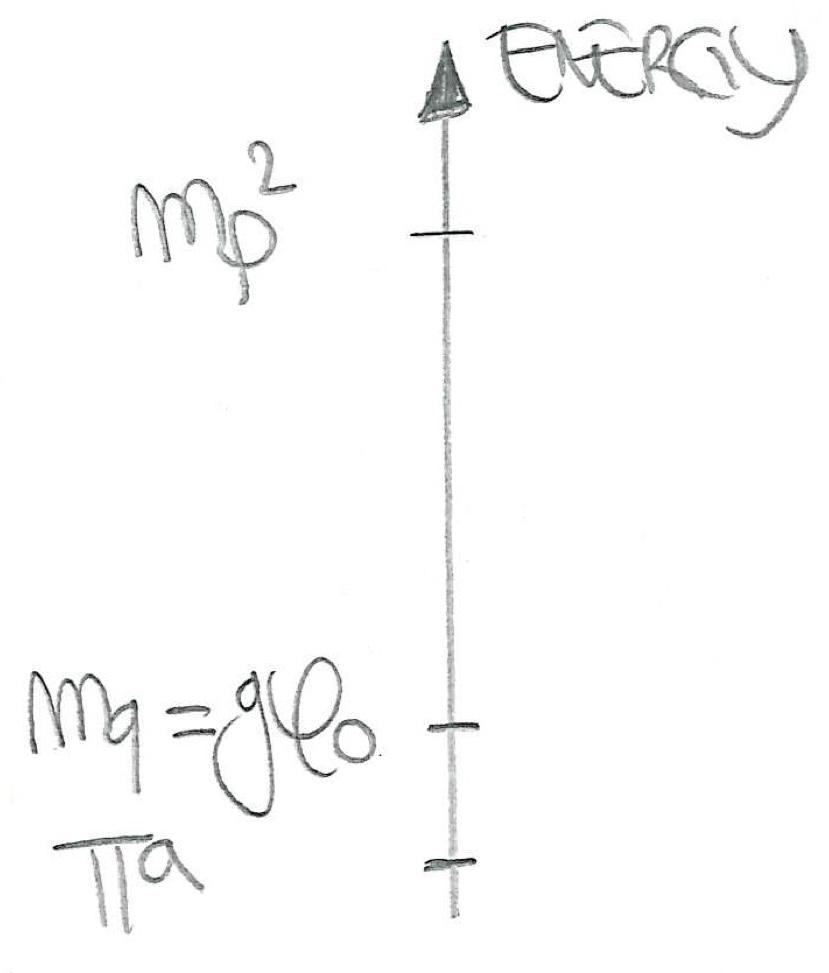
\includegraphics[]{images_ch9/rhodecoupling.jpg}}
    \textbf{Al contrario, $\rho$ è un singoletto e non contiene alcuna informazione in merito al pattern di rottura di simmetria.}
\end{itemize}

Cerchiamo di esplicitare l'affermazione appena fatta considerando il limite in cui $\mu^2\rightarrow\infty$ e $\lambda\rightarrow\infty$, così che $\varphi_0^2 = \frac{\mu^2}{\lambda} = const.$ .

In tale limite anche la massa $m_\rho\rightarrow \infty$ e il campo radiale si disaccoppia dalle componenti di bassa energia della teoria, nel senso che (siccome per produrre una particella $\rho$ con una certa massa $m_\rho$ è necessario avere a disposizione almeno il doppio di questa massa come energia del centro di massa) nel limite di $m_\rho$ molto grande, non c'è modo di produrre $\rho$. Avrebbe quindi senso “eliminare” tale campo dalla Lagrangiana o, per meglio dire, “\textbf{integrarlo fuori}”.

Definiamo quindi la procedura da seguire per effettuare tale operazione, che si compone di tre step:
\marginnote{La logica del punto ii) si ritrova nel fatto che siamo interessati al caso in cui $\lambda$ è molto grande. Questo produce automaticamente un parametro molto piccolo nella teoria, pari esattamente all'inverso di $\lambda$}
\begin{enumerate}
    \item[\textbf{i)}] Scriviamo l'equazione del moto per $\rho$.
    \item[\textbf{ii)}] Espandiamo la soluzione in potenze di $\frac{1}{\lambda}$.
    \item[\textbf{iii)}] Utilizziamo la soluzione ricavata nel punto ii) nella Lagrangiana.
\end{enumerate}

Ora sviluppiamo questi passaggi:
\begin{enumerate}
    \item[\textbf{i)}] \textbf{Equazione del moto per $\rho$.}

    Le equazioni del moto sono definite da $\partial_\mu\frac{\partial\mathscr L}{\partial(\partial_\mu\rho)} = \frac{\partial\mathscr L}{\partial\rho}$ e non è difficile convincersi del fatto che in questo caso questa equazione si riduca a:
    \begin{equation}
        \boxed{\Box\rho +2\varphi_0^2\lambda\rho + 3\varphi_0\lambda\rho^2 + \lambda\rho^3 - \frac{(\rho+\varphi_0)}{2}t - \mathsf g\big(\bar q_L U q_R + \bar q_R U^\dagger q_L\big)= 0}
        \label{eq:rho_EoM}
    \end{equation}
    dove $t \equiv \Tr\big[\big(\partial_\mu U\big)\big(\partial^\mu U^\dagger\big)]$ e si è usato $\mu^2 = \varphi_0^2\lambda$ e $\mu=\varphi_0\sqrt\lambda$
    
    \item[\textbf{ii)}] \textbf{Soluzione in potenze di $\frac{1}{\lambda}$.}

    L'idea è quella di riscrivere il campo radiale come 
    \[\rho = \rho_0 +\frac{1}{\lambda}\rho_1 + \cdots\] 
    e per farlo procediamo in maniera iterativa.

    \underline{Ad $\mathscr O(\lambda^1)$}, il più alto ordine di $\lambda$, la (\ref{eq:rho_EoM}) si riduce a:
    \[
    2\varphi_0\lambda\rho_0 + 3\varphi_0\lambda\rho_0^2 +\lambda\rho_0^3 = 0 \Rightarrow ~ \boxed{\rho_0 = 0}
    \]
    Ed ha senso: $\rho$ produce le eccitazioni radiali attorno a $\varphi_0$ ma non abbiamo energia a sufficienza per produrlo nel limite di bassa energia, quindi nel momento in cui ci accontentiamo dell'ordine minore dell'espansione che stiamo considerando non abbiamo modo di deviare radialmente da $\varphi_0$.
    
    quindi possiamo già dire che $\rho = 0 + \frac{1}{\lambda}\rho_1$.

    \underline{Ad $\mathscr O(\lambda^0)$} abbiamo dunque:
    \begin{align*}
        &2\varphi_0^2\Ccancel[blue]{\lambda}\frac{\rho_1}{\Ccancel[blue]{\lambda}} - \frac{(\Ccancel[Red]{\rho_0}+\varphi_0)}{2}t- \mathsf g\big(\bar q_L U q_R + \bar q_R U^\dagger q_L\big) = 0\\
        &2\varphi_0^2\rho_1 = \frac{\varphi_0}{2}t + \mathsf g\big(\bar q_L U q_R + \bar q_R U^\dagger q_L\big)\\
        &\rho_1 = \frac{1}{4\varphi_0}t + \frac{\mathsf g}{2\varphi_0^2}\big(\bar q_L U q_R + \bar q_R U^\dagger q_L\big)
    \end{align*}
    dunque la soluzione ad $\mathscr O\big(\frac{1}{\lambda}\big)$:
    \begin{equation}
        \boxed{\rho = \frac{1}{4\varphi_0\lambda}t + \frac{\mathsf g}{2\varphi_0^2\lambda}\big(\bar q_L U q_R + \bar q_R U^\dagger q_L\big) + \mathscr O\bigg(\frac{1}{\lambda^2}\bigg)}
        \label{eq:rho_order1/lambda}
    \end{equation}
    
    \item[\textbf{iii)}] \textbf{Soluzione ricavata nella Lagrangiana.}

    Questo passaggio, al prim'ordine, corrisponde a fissare $\rho = \rho_0 = 0$ nella \ref{eq:nonlinear_lagrangian_SU2_V+fermions}, ottenendo la Lagrangiana “Low-Energy”:
    \begin{equation}
        \boxed{\mathscr{L}_\text{LE} = \bar q i\gamma^\mu\partial_\mu q + \frac{\varphi_0^2}{4}\Tr\big[\big(\partial_\mu U\big)\big(\partial^\mu U^\dagger\big)] + \mathsf{g}\varphi_0\big(\bar q_L U q_R + \bar q_R U^\dagger q_L\big)}
        \label{eq:leadingorder_lagrangian_rho_intout}
    \end{equation}
\end{enumerate}

\textbf{In sintesi:} a bassa energia, integrando fuori il campo radiale, note le proprietà di trasformazione dei campi di Goldstone sotto l'azione del gruppo di simmetria completo (determinate dalla forma infinitesima di $U\rightarrow LUR^\dagger$), \textbf{la struttura della Lagrangiana è completamente determinata dal pattern di rottura di simmetria SU$\mathbf{(2)_L\times}$SU$\mathbf{(2)_R\rightarrow}$SU$\mathbf{(2)_V}$}, nel senso che gli unici termini che possiamo scrivere nella Langrangiana sono quelli che rispettano la simmetria sotto $U = \exp(i\pi^a\sigma^a/f_\pi)$.

\begin{nota}
    Quanto appena osservato, riguardo la struttura a bassa energia di una teoria che subisce una rottura spontanea di simmetria, è rilevante soprattutto perché, in generale, non conosciamo quale sia la teoria completa.
\end{nota}
\begin{exercise}
    Calcolare la forma esplicita della Lagrangiana ad $\mathscr O\big(\frac{1}{\lambda}\big)$. \textbf{[Conti svolti Lez. 38.1 p. 101÷102]}
\end{exercise}
\end{document}
$\boxed{}$

\begin{figure}[h]
    \centering
    \includegraphics{images/semplicementepanati.png}
    \caption*{}
    \label{fig:my_label}
\end{figure}